\documentclass[
]{elteikthesis}[2023/04/10]

\title{Multimodal Pneumonia Detection from Chest X-rays and Clinical Data using MIMIC-CXR and MIMIC-IV}
\date{2026}

\author{Yazan Al-Dabain}
\degree{Computer Science BSc}

\supervisor{Dr Arafat Md Easin}
\affiliation{Assistant Lecturer}

\university{Eötvös Loránd University}
\faculty{Faculty of Informatics}
\department{Dept. of Software Technology and Methodology}
\city{Budapest}
\logo{elte_cimer_szines}

\addbibresource{references.bib}

\usepackage{tikz}
\usepackage{longtable}
\usepackage{array}
\usepackage{booktabs}
\usepackage{verbatim}
\usetikzlibrary{calc, positioning, arrows.meta}

\begin{document}

\documentlang{english}

\maketitle
\tableofcontents
\cleardoublepage

\chapter{Introduction}

Pneumonia is frequently evaluated in acute care using chest radiography. Chest X-rays (CXR) are typically acquired early in the clinical encounter when pulmonary infection is suspected, making them a natural anchor point for predictive modeling. Automated analysis of CXR, particularly when combined with structured clinical data, has therefore become an active area of research. However, the validity of such models depends critically on whether their inputs and evaluation protocols reflect the actual information available at the intended prediction time.

Deep learning approaches, especially convolutional neural networks, have demonstrated strong performance in image-based chest pathology classification. In parallel, models built on structured tabular data—such as emergency department (ED) triage measurements—capture physiological and demographic information available at presentation. Combining these modalities is a natural extension when both are available for the same encounter. Nonetheless, the benefit of multimodal fusion is not guaranteed: it depends on the presence of complementary signal and on the strictness of the temporal constraints imposed on the input features. In particular, distinguishing pneumonia from other radiographic abnormalities—such as pleural effusion, pulmonary edema, or non-specific opacities—is inherently challenging, as these conditions often exhibit overlapping visual patterns on chest radiographs.

In this thesis, prediction is explicitly anchored at the time of image acquisition ($t_0$). Only variables available at or before $t_0$ are permitted as inputs. This constraint addresses a key challenge in medical machine learning, namely temporal leakage, where features reflecting downstream clinical decisions or outcomes may inadvertently be used during training. While restricting inputs to a pre-imaging window reduces the amount of available information and may increase task difficulty, it ensures that the problem formulation aligns with a clearly defined and clinically meaningful decision point.

The study is based on the MIMIC-CXR-JPG (v2.1.0) dataset and structured data from MIMIC-IV and MIMIC-IV-ED. An emergency department (ED)-linked cohort of chest radiograph studies is constructed under strict linkage and filtering criteria, including the selection of a single frontal image per study with deterministic prioritization and linkage to a corresponding ED stay for each retained study. The supervised task is binary radiographic pneumonia (target T1), derived from CheXpert labels using a \texttt{u\_ignore} uncertain-label policy, where uncertain labels are excluded from training and evaluation. It is important to note that this label reflects radiographic interpretation rather than a definitive etiologic diagnosis. The final labeled dataset contains 9{,}137 studies, partitioned using a patient-level temporal split into training, validation, and test sets.

Implemented models include triage-based clinical baselines (logistic regression and gradient boosted trees), an image-only DenseNet121 model fine-tuned for pneumonia following multilabel pretraining, and an early-fusion multimodal model combining image and clinical features. All models are trained and evaluated on a shared cohort under identical temporal constraints to enable direct comparison.

Evaluation is performed on a shared held-out temporal test set of 1{,}075 studies using discrimination metrics (AUROC and AUPRC), complemented by patient-level bootstrap resampling for paired comparisons. Additional analyses include calibration assessment, decision curve analysis (DCA), and error-oriented evaluations such as CheXpert-based stratification of negative cases and gradient-based visualizations for model interpretability. DCA is interpreted in a threshold-dependent manner, reflecting variation in clinical utility across operating points.

Within this setup, image-based models achieve higher discrimination than clinical baselines (AUROC 0.746 vs 0.595), while multimodal fusion does not demonstrate a consistent improvement over the image-only model (AUROC 0.736 vs 0.746), with paired bootstrap comparisons indicating no statistically reliable advantage. Performance is further sensitive to the composition of negative cases, with reduced discrimination observed when negatives include studies with other radiographic abnormalities. This behavior highlights the inherent ambiguity of radiographic pneumonia detection and suggests that models may respond to general abnormality patterns rather than disease-specific features. These findings motivate a careful, constraint-aware interpretation of multimodal learning in this setting. This study represents a retrospective single-dataset benchmark under strict temporal constraints.

\section*{Contributions}

\begin{itemize}
    \item A reproducible pipeline for constructing an ED-linked chest radiograph cohort with prediction anchored at imaging time, including strict enforcement of pre-imaging feature availability and explicit handling of leakage-prone variables.
    
    \item A controlled comparison of clinical, image-based, and multimodal models on a shared patient-level temporal split derived from 9{,}137 labeled studies.
    
    \item A comprehensive evaluation framework incorporating discrimination metrics, patient-level bootstrap analysis, calibration assessment, and decision curve analysis to provide a multi-dimensional assessment of model performance.
    
    \item Empirical evidence that multimodal fusion does not provide a consistent performance gain over a strong image-only baseline under strict temporal constraints, highlighting the importance of problem formulation in multimodal learning.
    
    \item An analysis of error structure showing that model performance depends strongly on the definition of negative cases, with reduced discrimination in the presence of other radiographic abnormalities, reflecting the inherent ambiguity of pneumonia detection from chest X-rays.
\end{itemize}
\chapter{Related Work}

\section{Chest X-ray Pneumonia Detection}

A large body of work formulates chest radiograph analysis as a supervised visual classification problem, most commonly using convolutional neural networks trained on datasets that pair images with structured labels. Resources such as MIMIC-CXR and CheXpert are widely adopted due to their scale, standardized label ontology, and compatibility with deep learning workflows. A common approach is to train models on multiple radiographic findings using multilabel supervision and subsequently adapt them to a narrower clinical endpoint such as pneumonia. This strategy typically produces strong image-only baselines, which any multimodal system must match or exceed to justify additional complexity.

The present thesis follows this paradigm for the imaging branch. A DenseNet121 encoder is trained under CheXpert-style multilabel supervision with an explicit masking policy for uncertain labels, and subsequently fine-tuned for a binary pneumonia target consistent with the project’s label definition. This two-stage training strategy leverages broader radiographic signal during pretraining while aligning the final model with the specific downstream task.

\section{Clinical Prediction Models}

In parallel, a substantial body of literature focuses on predicting clinical outcomes from structured electronic health record data, including emergency department (ED) triage measurements. Linear models and tree-based ensembles remain widely used due to their interpretability, robustness to heterogeneous feature types, and ability to capture nonlinear relationships.

In this thesis, clinical baselines are implemented using logistic regression and gradient boosted trees (XGBoost). Logistic regression provides a transparent linear reference model, while XGBoost serves as a nonlinear baseline capable of modeling interactions between variables. Both models are trained on triage-derived features that reflect physiological state at presentation, under a strict feature policy that excludes variables not reliably available at the prediction time.

Triage-based predictors are inherently constrained by missingness, limited granularity, and the absence of visual information present in imaging. Additionally, clinical datasets often contain variables that may reflect downstream decisions rather than initial patient state. In this work, such variables—particularly disposition-related fields—are explicitly excluded to prevent temporal leakage and ensure that all features correspond to information available at or before the prediction time.

\section{Multimodal Learning in Medical Imaging}

Multimodal learning aims to combine imaging and non-imaging data when both are available for the same clinical encounter. Early fusion approaches, which integrate learned image representations with tabular features into a joint model, are a common and practical strategy for single-timepoint prediction settings.

In this thesis, multimodal fusion is implemented using an early-fusion architecture in which features extracted from the image encoder are combined with tabular clinical representations through feature concatenation and jointly optimized. Conceptually, clinical variables may provide complementary information not fully captured by the radiograph, particularly in representing physiological context.

However, empirical evidence across studies suggests that improvements from multimodal fusion are not consistently observed, especially when strong image baselines are used. The benefit of multimodal integration therefore cannot be assumed a priori and must be evaluated under controlled conditions. In particular, when clinical features are restricted to pre-imaging triage data, the incremental signal available to the multimodal model may be limited, making performance gains over image-only models uncertain.

\section{Limitations of Prior Work}

Several limitations recur in prior work and complicate the interpretation of reported performance. A common issue is the absence of a clearly defined prediction time, leading to pipelines that incorporate variables whose temporal relationship to the imaging study is ambiguous. When predictors include information influenced by events after image acquisition, such as documentation or disposition-related fields, models may inadvertently exploit future information. This form of temporal leakage can lead to overly optimistic estimates of performance, particularly in multimodal settings where heterogeneous data sources are combined.

Beyond temporal concerns, many studies do not enforce patient-level temporal splits or provide paired uncertainty estimates when comparing models. As a result, reported performance differences may not reflect statistically meaningful improvements. Additionally, calibration and decision-oriented evaluations are often omitted, limiting insight into how models would behave in practical settings. Discrimination metrics alone do not capture the reliability of predicted probabilities or their clinical utility, and different models may exhibit trade-offs between discrimination and calibration. Furthermore, clinical utility is inherently threshold-dependent, meaning that no single model may be optimal across all decision thresholds.

Finally, report-derived labels such as those from CheXpert introduce inherent uncertainty and ambiguity. Pneumonia is defined within a broader multilabel ontology, uncertain annotations are common, and negative labels do not necessarily correspond to radiographically normal studies. Consequently, model performance can depend strongly on how negative cases are defined. In particular, distinguishing pneumonia from other abnormal radiographic findings is substantially more difficult than distinguishing it from normal studies, highlighting the importance of analyzing performance across different negative case compositions.

These limitations directly motivate the design of this thesis. The problem is formulated with prediction anchored at the time of image acquisition ($t_0$), ensuring that only pre-imaging information is used. Clinical features are restricted to triage data to prevent temporal leakage, and all models are evaluated on a shared patient-level temporal split to enable fair comparison. Model performance is assessed not only through discrimination metrics, but also through paired bootstrap analysis, calibration evaluation, decision curve analysis, and error-oriented diagnostics. Within this framework, the central question is whether multimodal fusion provides a reliable incremental benefit over a strong image-only baseline under strict temporal and data availability constraints.
\chapter{Data and Cohort Construction}

\section{Data Sources}

The imaging data are drawn from MIMIC-CXR-JPG (version~2.1.0). Structured clinical inputs are derived from MIMIC-IV-ED, specifically emergency department (ED) stay records and triage tables used in cohort linkage and feature construction. The broader MIMIC-IV database is present in the repository for auxiliary pipelines (e.g., laboratory data), but the primary experiments in this thesis rely exclusively on ED-linked chest radiographs and triage features.

The full data processing pipeline is implemented as a sequence of deterministic scripts, including cohort construction, ED linkage, temporal splitting, and downstream table generation. Key steps are executed through scripts such as \texttt{build\_primary\_imaging\_cohort.py}, \texttt{link\_cxr\_to\_edstays.py}, \texttt{build\_final\_ed\_cohort.py}, and \texttt{build\_temporal\_patient\_split.py}. Configuration details for dataset access and local paths are defined in repository configuration files and are not hard-coded.

\section{Cohort Definition}

Cohort construction follows a deterministic pipeline starting from a chest radiograph manifest derived from MIMIC-CXR-JPG. Studies are restricted to frontal views (posteroanterior or anteroposterior), and a single image per study is selected, with posteroanterior priority when multiple candidates are available.

An imaging timestamp ($t_0$) is parsed from study date and time metadata and used as the temporal reference for all downstream processing. Missingness in $t_0$ is tracked during cohort construction; in the retained ED-linked cohort, no studies exhibit missing imaging timestamps.

Radiograph studies are linked to MIMIC-IV-ED emergency department stays using a temporal overlap rule:
\[
\texttt{intime} \leq t_0 \leq \texttt{outtime}.
\]
Only studies with exactly one matched ED stay are retained ($n_{\text{ed\_matches}} = 1$), ensuring a unique and unambiguous clinical context for each imaging study.

Additional integrity filtering removes rows with missing image paths where applicable. The resulting ED-linked cohort contains 81{,}385 studies from 47{,}404 patients and forms the parent population for all downstream label construction and model evaluation.

The filtering process used to derive the final benchmark cohort is summarized in Figure~\ref{fig:cohort_flow}. Starting from the full manifest, the pipeline restricts the data to frontal studies, performs ED linkage under temporal constraints, and retains the labeled subset used for model development and evaluation.

\begin{figure}[htbp]
    \centering
    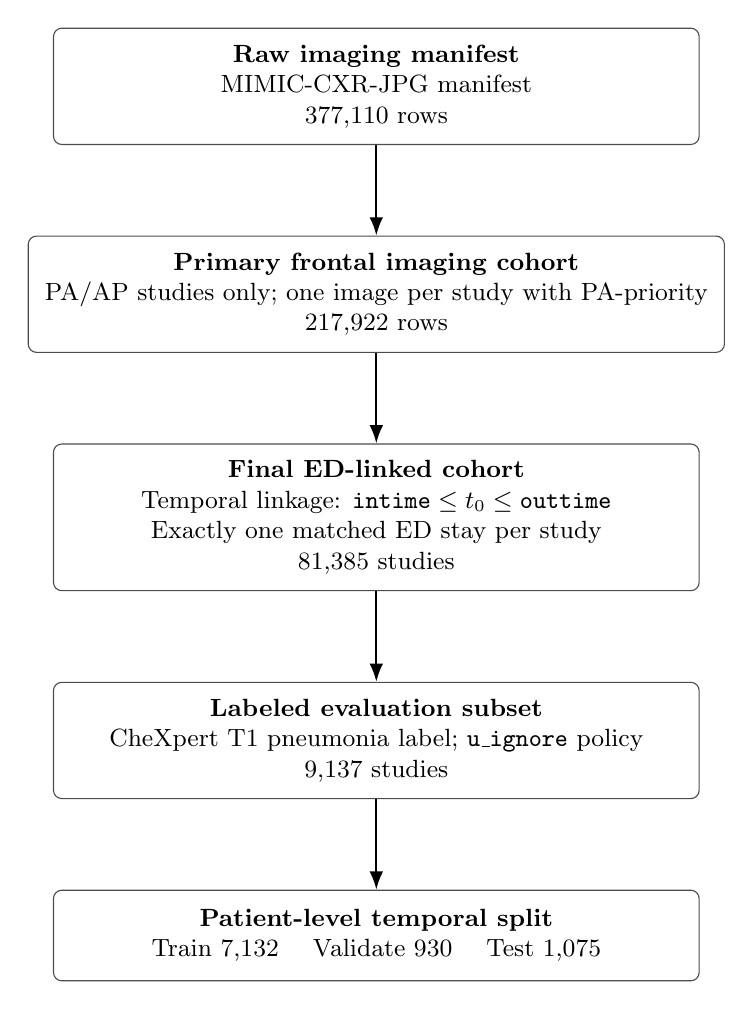
\begin{tikzpicture}[
        font=\small,
        >=Latex,
        node distance=1.15cm,
        box/.style={
            draw=black!70,
            rounded corners=3pt,
            align=center,
            minimum width=8.2cm,
            minimum height=1.15cm,
            inner sep=6pt
        },
        arrow/.style={->, thick}
    ]

    \node[box] (raw) {
        \textbf{Raw imaging manifest}\\
        MIMIC-CXR-JPG manifest\\
        377{,}110 rows
    };

    \node[box, below=of raw] (frontal) {
        \textbf{Primary frontal imaging cohort}\\
        PA/AP studies only; one image per study with PA-priority\\
        217{,}922 rows
    };

    \node[box, below=of frontal] (ed) {
        \textbf{Final ED-linked cohort}\\
        Temporal linkage: $\texttt{intime} \leq t_0 \leq \texttt{outtime}$\\
        Exactly one matched ED stay per study\\
        81{,}385 studies
    };

    \node[box, below=of ed] (label) {
        \textbf{Labeled evaluation subset}\\
        CheXpert T1 pneumonia label; \texttt{u\_ignore} policy\\
        9{,}137 studies
    };

    \node[box, below=of label] (split) {
        \textbf{Patient-level temporal split}\\
        Train 7{,}132 \quad Validate 930 \quad Test 1{,}075
    };

    \draw[arrow] (raw) -- (frontal);
    \draw[arrow] (frontal) -- (ed);
    \draw[arrow] (ed) -- (label);
    \draw[arrow] (label) -- (split);

    \end{tikzpicture}
    \caption{Cohort derivation for the primary benchmark. Starting from the full MIMIC-CXR-JPG manifest, the pipeline restricts the data to frontal studies, links studies to emergency department encounters using a temporal overlap rule, and retains the CheXpert-labeled \texttt{u\_ignore} subset used for model development and evaluation. Reported counts correspond to generated cohort reports in the pipeline artifacts.}
    \label{fig:cohort_flow}
\end{figure}

\section{Prediction Time and Feature Availability}

Prediction is anchored at the imaging time, defined as the chest radiograph acquisition timestamp ($t_0$). All model inputs are restricted to information available at or before this reference time. This constraint is enforced to align the prediction task with a well-defined clinical moment and to prevent the inclusion of variables influenced by future events.

For the clinical and multimodal baselines, features are limited to emergency department triage data. These include vital signs and scores (temperature, heart rate, respiratory rate, oxygen saturation, systolic and diastolic blood pressure, pain, and acuity), categorical variables (gender, race, arrival transport), and missingness indicators derived for numeric fields after plausibility filtering.

Free-text chief complaint is excluded from the baseline models, and disposition is explicitly removed due to its dependence on downstream clinical decisions and high leakage risk. Feature preprocessing, including scaling, encoding, and imputation, is fit exclusively on the training split within each modelling pipeline to prevent information leakage across splits.

\section{Label Definition}

The primary supervision target is radiographic pneumonia derived from the CheXpert label set (target~T1 in the project definition). Labels are merged into the cohort using study-level identifiers.

In the canonical pipeline run, labels are joined using \texttt{subject\_id} and \texttt{study\_id} as merge keys, reflecting a fallback strategy when image-level identifiers are not consistently available. Consistency checks are applied during the merge process to detect and resolve conflicts.

The primary label policy (\texttt{u\_ignore}) retains only definite positive and negative annotations and excludes uncertain cases. This results in a labeled subset of 9{,}137 studies used for model training and evaluation. An alternative policy (\texttt{u\_zero}) is implemented in the repository but is not used in the primary experiments.

\section{Dataset Splitting}

Data are partitioned using a patient-level temporal split. Each patient is assigned to a single split based on the timing of their earliest imaging study, and all subsequent studies from that patient inherit the same assignment. This ensures that no patient appears in more than one split and that evaluation reflects temporal generalization.

The temporal split is first constructed at the patient level on the full ED-linked cohort and is then propagated to labeled, imaging, and clinical tables using consistent study-level keys. This guarantees that all model variants are trained and evaluated on identical data partitions.

For the primary labeled dataset (\texttt{u\_ignore}), the resulting split contains 7{,}132 training, 930 validation, and 1{,}075 test studies. The combination of patient-level partitioning and strict feature timing constraints is intended to minimize both subject leakage and temporal leakage in model evaluation.
\chapter{Methods}

\section{Overview}

This chapter describes the modelling and evaluation procedures used in the thesis. Three families of models are trained and evaluated on the same temporally split cohort described previously. Clinical baselines use only emergency department (ED) triage--derived tabular inputs. The image model is a DenseNet121 classifier trained on chest radiographs. The multimodal model applies early fusion by concatenating a pooled visual embedding with an encoded tabular representation and passing the result through a feedforward classifier. All supervised training uses the same binary pneumonia target and the predefined training, validation, and test partitions.

The methodological design is intentionally aligned with the thesis objective of evaluating multimodal learning under realistic temporal constraints. In particular, all model families operate on data derived from the same ED-linked cohort, the same pneumonia label policy, and the same patient-level temporal split. This shared setup ensures that performance differences can be interpreted primarily as differences in model family and input modality, rather than as artifacts of inconsistent cohort construction or evaluation design.

Figure~\ref{fig:pipeline_overview} summarizes the end-to-end pipeline used in this thesis, from data sources and cohort construction to model training and evaluation.

\begin{figure}[htbp]
    \centering
    \resizebox{\textwidth}{!}{%
    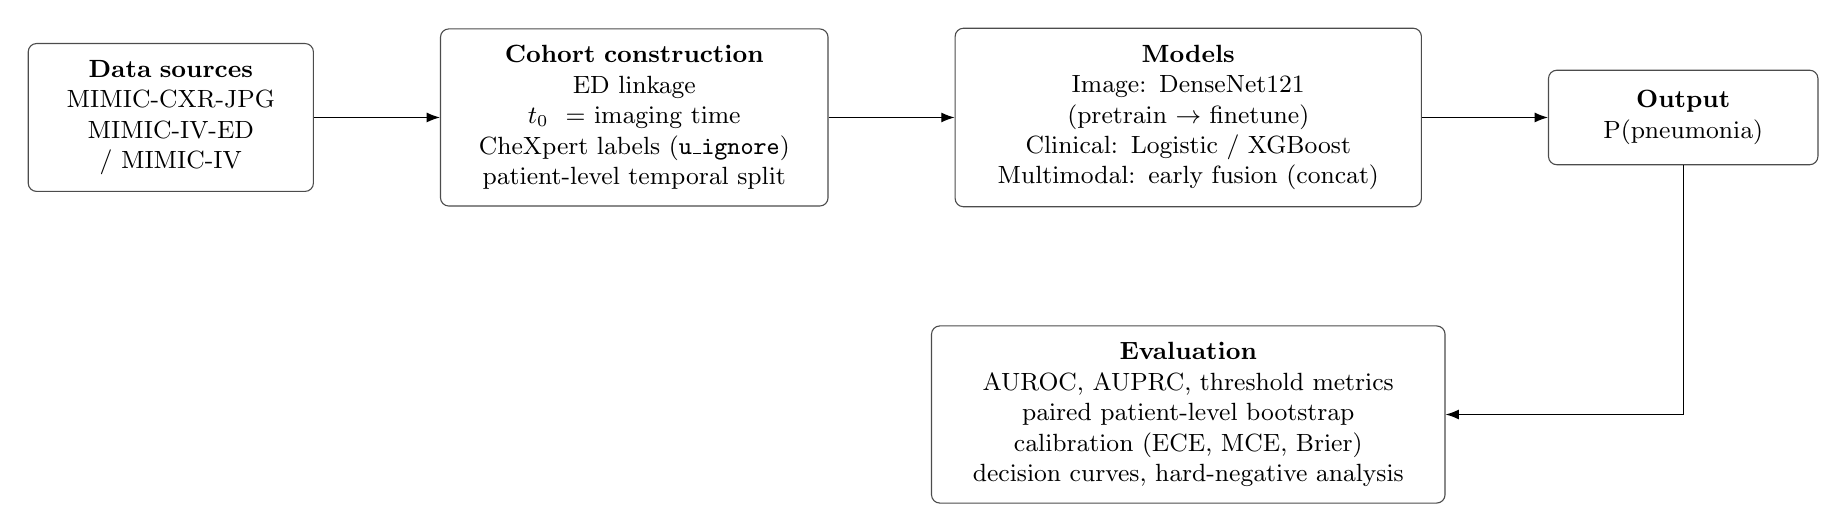
\begin{tikzpicture}[
        font=\small,
        >=Latex,
        node distance=1.6cm,
        box/.style={
            draw=black!70,
            rounded corners=3pt,
            align=center,
            inner sep=6pt,
            minimum height=1.2cm
        }
    ]
    
    % --- DATA ---
    \node[box, text width=3.2cm] (data) {
    \textbf{Data sources}\\
    MIMIC-CXR-JPG\\
    MIMIC-IV-ED / MIMIC-IV
    };
    
    % --- COHORT ---
    \node[box, text width=4.5cm, right=of data] (cohort) {
    \textbf{Cohort construction}\\
    ED linkage\\
    $t_0 =$ imaging time\\
    CheXpert labels (\texttt{u\_ignore})\\
    patient-level temporal split
    };
    
    % --- MODELS ---
    \node[box, text width=5.5cm, right=of cohort] (models) {
    \textbf{Models}\\
    Image: DenseNet121 (pretrain $\rightarrow$ finetune)\\
    Clinical: Logistic / XGBoost\\
    Multimodal: early fusion (concat)
    };
    
    % --- OUTPUT ---
    \node[box, text width=3.0cm, right=of models] (out) {
    \textbf{Output}\\
    P(pneumonia)
    };
    
    % --- EVAL ---
    \node[box, text width=6.1cm, below=1.5cm of models] (eval) {
    \textbf{Evaluation}\\
    AUROC, AUPRC, threshold metrics\\
    paired patient-level bootstrap\\
    calibration (ECE, MCE, Brier)\\
    decision curves, hard-negative analysis
    };
    
    % --- ARROWS ---
    \draw[->] (data) -- (cohort);
    \draw[->] (cohort) -- (models);
    \draw[->] (models) -- (out);
    \draw[->] (out) |- (eval);
    
    \end{tikzpicture}%
    }
    \caption{Overview of the pneumonia detection pipeline. Data are used to construct a temporally aligned cohort anchored at imaging time ($t_0$). Clinical, image-only, and multimodal models are trained and evaluated using multiple complementary metrics and uncertainty analysis.}
    \label{fig:pipeline_overview}
\end{figure}

The stages in Figure~\ref{fig:pipeline_overview} mirror the data construction described in the previous chapter and the training and evaluation procedures detailed in the subsections below.

\section{Clinical Models}

The clinical branch is designed to provide interpretable tabular baselines based exclusively on information available at or before the imaging time. These models serve two purposes. First, they quantify how much signal is available from structured triage data alone. Second, they provide a reference point against which the image-only and multimodal systems can be compared.

Two tabular baselines share identical feature sets. Numeric inputs include vital signs, missingness indicators, and the binary view flags \texttt{is\_pa} and \texttt{is\_ap}. Categorical inputs include \texttt{gender}, \texttt{race}, and \texttt{arrival\_transport}. Numeric features are cast to floating point with missing values retained for imputation. Missingness indicators are filled to one when absent, while view flags are filled to zero. Categorical variables are normalized to string representations, with unknown categories mapped to a dedicated token. This preprocessing strategy ensures that missingness is represented explicitly rather than silently absorbed into imputed values, which is especially important in clinical data.

The first baseline is logistic regression. It is implemented as a preprocessing pipeline followed by an L2-regularized classifier with the SAGA solver, a maximum of ten thousand iterations, and balanced class weights. Numeric features are median-imputed and standardized, while categorical features are imputed with a constant token and one-hot encoded with unknown categories ignored at transform time. The pipeline is fit on the training split only and applied unchanged to validation and test data. This model is intentionally simple and serves as a strong linear reference for the triage feature space.

The second baseline is a gradient-boosted tree model implemented using XGBoost with native categorical handling. The classifier uses a binary logistic objective with \texttt{n\_estimators=2000}, \texttt{max\_depth=5}, \texttt{learning\_rate=0.03}, \texttt{subsample=0.8}, \texttt{colsample\_bynode=0.8}, \texttt{reg\_lambda=1}, \texttt{tree\_method="hist"}, \texttt{enable\_categorical=True}, \texttt{n\_jobs=-1}, and \texttt{random\_state=42}. Categorical variables are converted to pandas categorical type before fitting. Training proceeds with early stopping after forty rounds without improvement on validation AUPRC. The positive class weight is set to the ratio of negative to positive examples in the training data using \texttt{scale\_pos\_weight}. Relative to logistic regression, this model is intended to capture nonlinear relationships and higher-order interactions among triage variables while remaining computationally lightweight and interpretable at a system level.

Taken together, the two clinical baselines define a tabular-only performance envelope for the task. If the image model substantially exceeds them, then the radiograph clearly contains additional signal. If multimodal learning improves over both the image and clinical baselines, that improvement can more credibly be attributed to complementary cross-modal information rather than weak unimodal modelling.

\section{Image Model}

The image model is based on torchvision DenseNet121 initialized with ImageNet weights. DenseNet121 is selected because it provides a strong and well-established convolutional backbone for chest radiograph analysis while remaining computationally manageable in the local training environment. The classifier head is replaced with a linear layer producing a single logit for binary pneumonia prediction. Input images are resized to a fixed square resolution (default 224 pixels), converted to tensors, and normalized using ImageNet statistics.

The imaging branch is trained in two stages: multilabel pretraining followed by task-specific fine-tuning. This design reflects the fact that radiographic pneumonia is not an isolated visual phenomenon but one component of a broader pathology space. Pretraining on multiple chest radiograph findings encourages the backbone to learn more general thoracic representations before specialization to the binary pneumonia task.

For multilabel pretraining, the classifier head is replaced with a multi-output linear layer corresponding to the selected CheXpert labels. Training uses masked binary cross-entropy with logits, where only observed binary labels contribute to the loss. In practice, only entries with valid observed \(0/1\) supervision contribute to optimization, while uncertain and missing labels are masked out. This masking strategy is important because CheXpert-style supervision contains uncertain and missing entries, and these should not be treated identically to observed negative labels.

Optimization during pretraining is performed using AdamW with separate learning rates for backbone and classifier parameters, weight decay of 0.0001, optional mixed-precision training, and gradient clipping. Data augmentation at this stage includes horizontal flipping, small rotations, and mild Gaussian blur. Learning rate scheduling follows a ReduceLROnPlateau strategy. By default, model selection in pretraining is based on validation masked loss (\texttt{val\_loss}), although alternative validation criteria such as micro-averaged AUPRC are supported in the training code. The default pretraining budget is 30 epochs with early stopping patience of 5 epochs without improvement.

Fine-tuning for pneumonia initializes from ImageNet or an optional multilabel checkpoint, depending on the run configuration. When a pretrained checkpoint is used, backbone weights are loaded while the final classifier head is reinitialized for binary output. The fine-tuning loss is binary cross-entropy with logits, using a positive class weight computed from the training split as the ratio of negative to positive examples. Optimization, checkpointing, and learning rate scheduling follow the same general strategy as in pretraining, but model selection is based on validation AUPRC rather than validation loss. The default fine-tuning budget is 40 epochs with early stopping patience of 10 epochs. Compared with pretraining, data augmentation is lighter; the fine-tuning pipeline uses resize, normalization, and mild Gaussian blur rather than the full pretraining augmentation set.

AUPRC is emphasized because pneumonia prevalence in the labeled benchmark is not extremely low but still sufficiently imbalanced that area under the precision--recall curve provides a useful complement to AUROC for model selection and final evaluation.

This two-stage image-training strategy is intended to produce a strong unimodal radiograph baseline. In the context of this thesis, it also serves as the reference against which multimodal fusion must be judged. A central question is not simply whether multimodal learning works in absolute terms, but whether it improves on an already competitive image representation learned from the same cohort and evaluated under the same temporal constraints.

\section{Multimodal Model}

The multimodal architecture combines a DenseNet121 image encoder with a tabular multilayer perceptron. The design goal is to fuse radiographic and triage information while keeping the architecture simple, interpretable at a high level, and directly comparable to the unimodal baselines.

The image branch applies convolutional feature extraction followed by global average pooling to produce a 1024-dimensional embedding. This dimension is inherited directly from the DenseNet121 backbone. The tabular branch consists of a two-layer feedforward network with batch normalization, ReLU activations, and dropout, producing a 128-dimensional representation. The difference in dimensionality reflects the fact that the raw information content and representational complexity of the image branch are substantially larger than those of the structured triage branch.

Figure~\ref{fig:early_fusion_architecture} illustrates the early-fusion design used in this thesis.

\begin{figure}[htbp]
    \centering
    \resizebox{\textwidth}{!}{%
    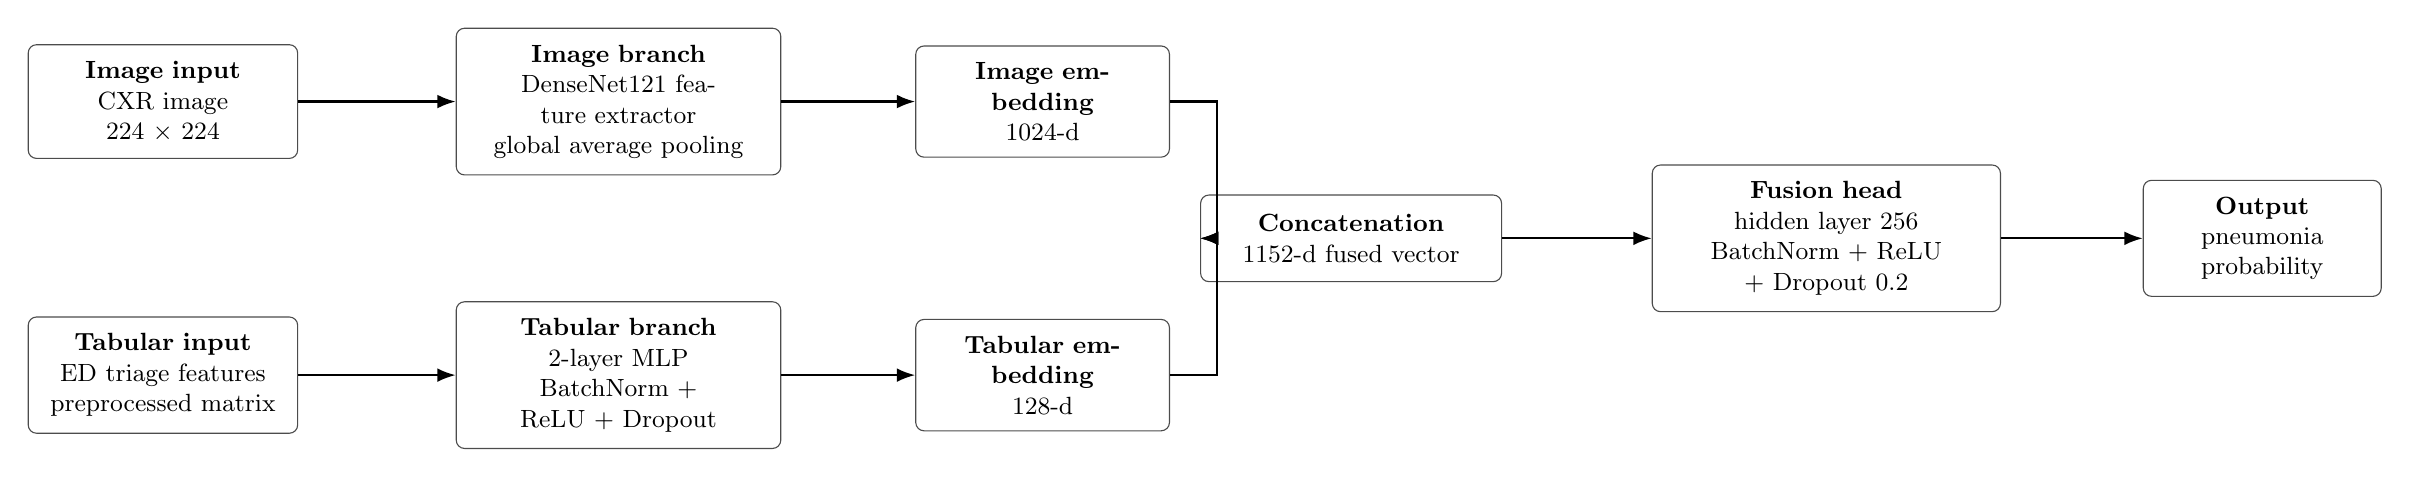
\begin{tikzpicture}[
        font=\small,
        >=Latex,
        node distance=1.4cm,
        box/.style={
            draw=black!70,
            rounded corners=3pt,
            align=center,
            minimum height=1.1cm,
            inner sep=6pt
        },
        arrow/.style={->, thick}
    ]

    % Inputs
    \node[box, text width=3.0cm] (imgin) {
        \textbf{Image input}\\
        CXR image\\
        224 $\times$ 224
    };

    \node[box, text width=3.0cm, below=2.0cm of imgin] (tabin) {
        \textbf{Tabular input}\\
        ED triage features\\
        preprocessed matrix
    };

    % Branches
    \node[box, text width=3.7cm, right=2.0cm of imgin] (imgenc) {
        \textbf{Image branch}\\
        DenseNet121 feature extractor\\
        global average pooling
    };

    \node[box, text width=3.7cm, right=2.0cm of tabin] (tabenc) {
        \textbf{Tabular branch}\\
        2-layer MLP\\
        BatchNorm + ReLU + Dropout
    };

    % Embeddings
    \node[box, text width=2.8cm, right=1.7cm of imgenc] (imgemb) {
        \textbf{Image embedding}\\
        1024-d
    };

    \node[box, text width=2.8cm, right=1.7cm of tabenc] (tabemb) {
        \textbf{Tabular embedding}\\
        128-d
    };

    % Fusion
    \node[box, text width=3.4cm, right=2.0cm of $(imgemb)!0.5!(tabemb)$] (concat) {
        \textbf{Concatenation}\\
        1152-d fused vector
    };

    \node[box, text width=4.0cm, right=1.9cm of concat] (fusion) {
        \textbf{Fusion head}\\
        hidden layer 256\\
        BatchNorm + ReLU + Dropout 0.2
    };

    \node[box, text width=2.6cm, right=1.8cm of fusion] (out2) {
        \textbf{Output}\\
        pneumonia probability
    };

    % Arrows
    \draw[arrow] (imgin) -- (imgenc);
    \draw[arrow] (tabin) -- (tabenc);

    \draw[arrow] (imgenc) -- (imgemb);
    \draw[arrow] (tabenc) -- (tabemb);

    \draw[arrow] (imgemb.east) -- ++(0.6,0) |- (concat.west);
    \draw[arrow] (tabemb.east) -- ++(0.6,0) |- (concat.west);

    \draw[arrow] (concat) -- (fusion);
    \draw[arrow] (fusion) -- (out2);

    \end{tikzpicture}%
    }
    \caption{Early-fusion multimodal architecture used in this thesis. A DenseNet121 image branch produces a 1024-dimensional visual embedding, while a two-layer multilayer perceptron encodes tabular triage features into a 128-dimensional representation. The two embeddings are concatenated into a 1152-dimensional fused vector and passed through a fusion head to generate the final pneumonia probability.}
    \label{fig:early_fusion_architecture}
\end{figure}

Early fusion is implemented by concatenating the image and tabular embeddings and passing the result through a fusion head comprising a fully connected layer, normalization, activation, dropout, and a final linear output layer. In the implemented model, the concatenated vector has dimensionality 1152 and is projected through a fusion hidden layer of size 256 before the final binary output. The default dropout rate in both the tabular and fusion branches is 0.2. This architecture is intentionally modest in complexity. Its purpose is not to exhaust the full space of multimodal architectures, but rather to provide a clean and well-defined test of whether triage information adds useful signal when fused with a strong image encoder under realistic timing constraints.

Tabular inputs are preprocessed using a column-wise transformer fitted on the training split, with median imputation and scaling for numeric features and constant imputation plus one-hot encoding for categorical features. This preprocessing is performed independently of the image branch but within the same split discipline as the clinical baselines, thereby preserving comparability and avoiding train--test leakage. The fitted tabular preprocessor is saved as an artifact (\texttt{tabular\_preprocessor.joblib}) to ensure reproducible transformation at validation and test time.

The image backbone may be initialized from ImageNet or a pretrained checkpoint. An optional configuration allows freezing backbone parameters so that only the tabular branch and fusion head are trained. When the backbone is trainable, optimization uses separate parameter groups for backbone and non-backbone components. In the main reported experiments, the multimodal model is trained under the same general evaluation framework as the image-only model so that the performance difference can be interpreted primarily as the effect of adding the tabular modality. The default multimodal training budget is 30 epochs with early stopping patience of 8 epochs, and model selection is based on validation AUPRC. As in the image fine-tuning stage, image preprocessing for multimodal training uses resize, normalization, and mild blur rather than the full augmentation set used during multilabel pretraining.

\section{Training Procedure}

All models are trained on the training partition and evaluated on validation and test partitions without cross-contamination. Neural models use mini-batch training with shuffled training data and deterministic validation and test evaluation. This common split discipline is essential because the thesis focuses not only on absolute performance but also on fair comparison across modalities.

Class imbalance is addressed differently for the three model families. Logistic regression uses balanced class weights. XGBoost uses \texttt{scale\_pos\_weight} computed from the training split. Neural models use weighted binary cross-entropy, with a positive class weight derived from the prevalence of the training labels. These strategies are intended to reduce bias toward the negative class without changing the underlying target definition.

Validation performance guides model selection throughout the system, but the exact criterion differs by training stage. Multilabel pretraining defaults to validation masked loss, whereas image fine-tuning and multimodal training both use validation AUPRC as the primary model-selection criterion. Neural models adjust learning rates when performance plateaus and apply early stopping after a fixed patience. The best validation checkpoint is retained for final test evaluation. Clinical models use validation primarily for monitoring, while XGBoost additionally uses it for early stopping. This consistent reliance on the validation split prevents test-set feedback during model development.

At the implementation level, model outputs, validation histories, checkpoints, and test predictions are saved as artifacts so that later analyses can be run from frozen predictions rather than from repeated retraining. This is particularly important for calibration assessment, decision curve analysis, bootstrap evaluation, and qualitative inspection, all of which are performed on saved outputs to ensure consistency across model families. Saved run artifacts include configuration files, training histories, summary files, serialized models or preprocessors, and prediction CSVs for validation and test partitions.

\section{Evaluation}

Model performance is assessed primarily using AUROC and AUPRC computed from predicted probabilities. Accuracy, precision, recall, and F1 score are additionally reported using a fixed decision threshold of 0.5. All metrics are evaluated on held-out test data with both classes present.

Uncertainty is quantified using patient-level bootstrap resampling. Patients are sampled with replacement, and all associated studies are included in each replicate. Metrics are recomputed for each bootstrap sample, and summary statistics including mean, standard deviation, and percentile-based intervals are reported. This approach respects the grouped structure of the dataset and avoids treating correlated studies from the same patient as independent observations. Although the generic evaluation utilities support a default of 1000 bootstrap replicates, the canonical analyses reported in this thesis use 2000 replicates with a fixed random seed.

Model comparisons use paired bootstrap resampling, ensuring that each replicate evaluates both models on the same resampled patient set. In the implemented evaluation pipeline, prediction files are aligned by \texttt{subject\_id} and, when available, \texttt{study\_id}, and consistency checks are performed to ensure that merged rows correspond to identical targets before paired differences are computed. Differences in AUROC and AUPRC are summarized across replicates. In addition to confidence intervals, the evaluation reports the fraction of bootstrap replicates in which one model outperforms another; this quantity should be interpreted as a bootstrap replicate proportion rather than as a formal frequentist \(p\)-value.

Calibration is evaluated using Brier score and reliability-style binning of predicted probabilities. Expected calibration error (ECE) and maximum calibration error (MCE) are computed using 10 equal-width bins over the unit interval. Bootstrap resampling is also used to summarize uncertainty in calibration metrics. These analyses complement discrimination metrics by assessing whether predicted probabilities align with observed event frequencies.

In addition, decision curve analysis (DCA) is used to assess threshold-dependent net benefit across models. In the canonical evaluation, thresholds range from 0.01 to 0.99 using 99 evenly spaced points. Before DCA curves are computed, model prediction files are checked for row consistency so that threshold-wise comparisons are performed on aligned prediction sets. Decision curve analysis complements AUROC and AUPRC by evaluating whether a model would improve threshold-based decision making relative to simpler strategies such as treating all or treating none.

Finally, qualitative analyses are conducted using gradient-based visualization methods applied to representative cases. These are not treated as substitutes for quantitative evaluation, but as complementary diagnostics that help interpret model behavior in correct and incorrect predictions. All evaluation procedures operate on saved prediction files or saved model checkpoints to ensure consistency, reproducibility, and comparability across experiments.
\chapter{Experiments and Results}

\section{Experimental Setup}

All reported metrics are computed on the temporal test partition of the pneumonia cohort (1{,}075 studies), with a positive fraction of 0.453. Patient-level bootstrap summaries are based on 887 unique \texttt{subject\_id} values. Discrimination metrics are evaluated on the full test set, while operational metrics use a fixed probability threshold of 0.5. Image and multimodal models correspond to the \texttt{stronger\_lr\_v3} configuration, and clinical baselines correspond to the \texttt{strong\_v2} artifacts. Paired comparisons use identical alignment keys (\texttt{subject\_id}, \texttt{study\_id}) across merged prediction tables.

This evaluation setup is intentionally shared across all model families so that differences in performance can be attributed to model design and input modality rather than to changes in cohort definition, label policy, or split construction. In other words, the results reported in this chapter are meant to answer a controlled comparative question: how much predictive value is obtained from triage data alone, from chest radiographs alone, and from early fusion of both modalities under the same temporally constrained benchmark?

\section{Main Results}

Table~\ref{tab:main_results} reports AUROC, AUPRC, accuracy, precision, recall, and F1 on the test split. The image-only DenseNet121 model achieves the highest AUROC (0.746), AUPRC (0.724), accuracy (0.678), recall (0.659), and F1 (0.650). The multimodal model ranks second on AUROC (0.736) and AUPRC (0.714), and third on accuracy (0.670), recall (0.606), and F1 (0.624).

Both deep learning models substantially outperform the clinical baselines on AUROC and AUPRC. Clinical XGBoost slightly exceeds logistic regression across all reported metrics. At a threshold of 0.5, multimodal precision (0.644) is marginally higher than image precision (0.641), while image recall exceeds multimodal recall (0.659 versus 0.606).

\begin{table}[htbp]
\centering
\caption{Test-set performance at probability threshold 0.5. Values are point estimates on 1{,}075 studies.}
\label{tab:main_results}
\begin{tabular}{lcccccc}
\hline
Model & AUROC & AUPRC & Accuracy & Precision & Recall & F1 \\
\hline
Clinical logistic & 0.606 & 0.548 & 0.577 & 0.535 & 0.507 & 0.521 \\
Clinical XGBoost & 0.611 & 0.567 & 0.579 & 0.535 & 0.528 & 0.532 \\
Image DenseNet121 & 0.746 & 0.724 & 0.678 & 0.641 & 0.659 & 0.650 \\
Multimodal & 0.736 & 0.714 & 0.670 & 0.644 & 0.606 & 0.624 \\
\hline
\end{tabular}
\end{table}

\begin{figure}[htbp]
    \centering
    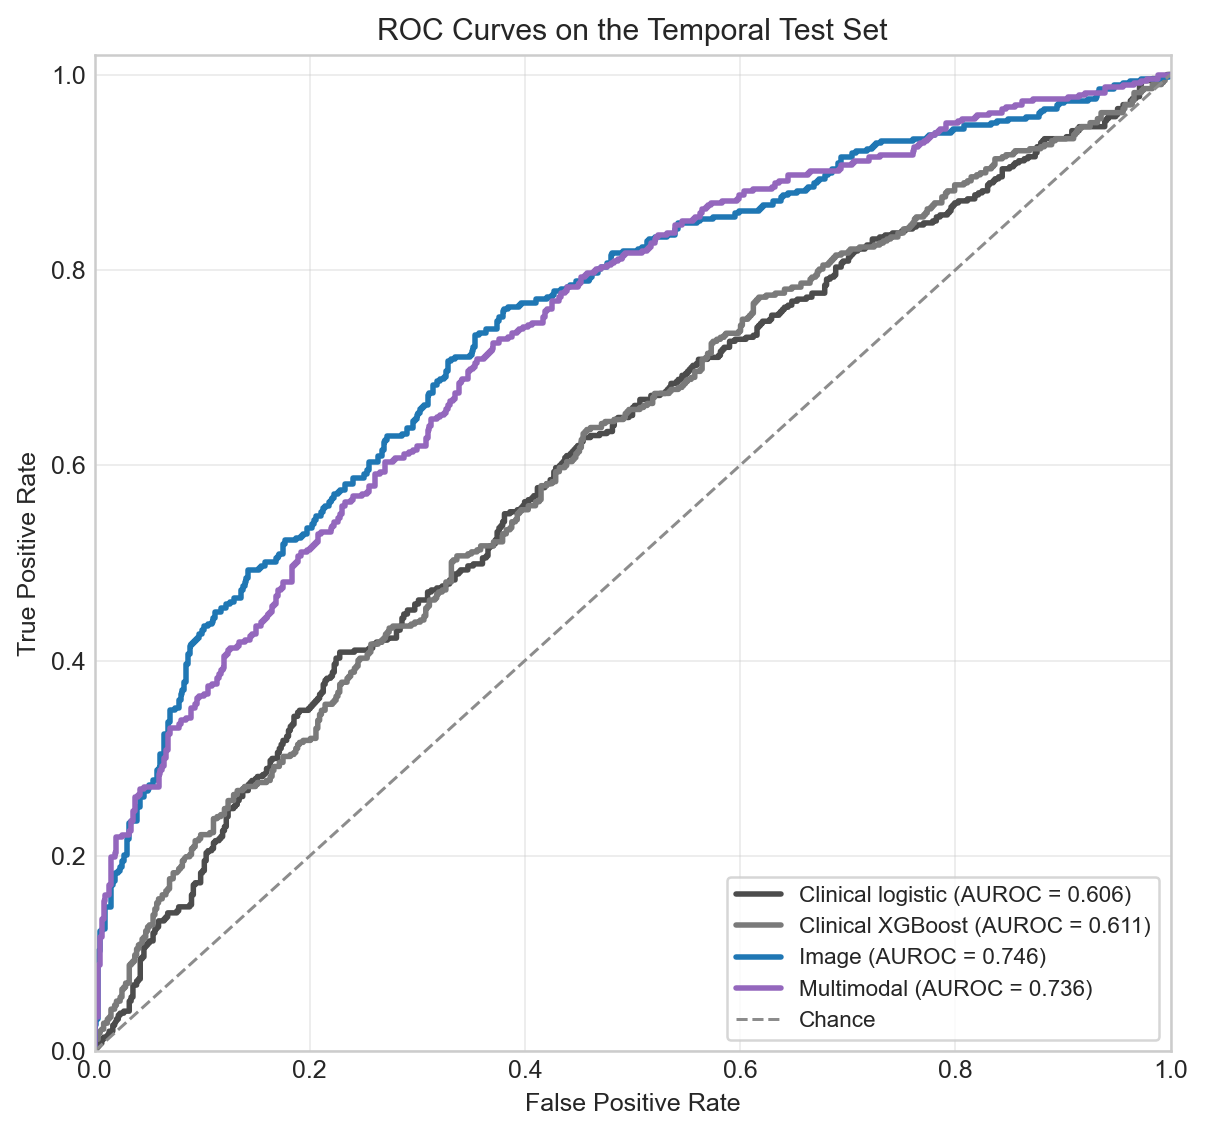
\includegraphics[width=0.8\textwidth]{images/roc_curve_all_models.png}
    \caption{Receiver operating characteristic (ROC) curves for the four evaluated models on the temporal test set. The image-only model achieves the highest discrimination performance (AUROC = 0.746), followed closely by the multimodal model (AUROC = 0.736), while both deep learning approaches substantially outperform the clinical baselines.}
    \label{fig:roc_all_models}
\end{figure}

The ROC curves for all evaluated models are shown in Figure~\ref{fig:roc_all_models}. The image-only model achieves the highest discrimination performance (AUROC = 0.746), with the multimodal model performing slightly worse (AUROC = 0.736).

Both deep learning approaches substantially outperform the clinical baselines (logistic regression: 0.606, XGBoost: 0.611). Importantly, the addition of clinical features via early fusion does not improve performance over the image-only model. This is the central empirical result of the thesis: under the current cohort design, label definition, and timing constraints, a strong radiograph model captures most of the useful signal available for the task.

The main result is therefore not simply that multimodal learning ``works,'' but that its benefit is limited in this setting. The multimodal model performs competitively in absolute terms and clearly exceeds the clinical-only baselines, yet it does not surpass the image-only baseline. This distinction is important because it shifts the interpretation from ``multimodal is better'' to ``multimodal should be justified empirically rather than assumed to be advantageous.''

\section{Uncertainty and Paired Comparisons}

Patient-level bootstrap with 2{,}000 replicates (seed 42) was applied to test predictions. For multimodal versus image, the mean paired differences were approximately $-0.0091$ AUROC (standard deviation $\approx 0.0070$) and $-0.0099$ AUPRC (standard deviation $\approx 0.0072$). The 95\% bootstrap intervals were $[-0.0227, 0.0047]$ for AUROC and $[-0.0240, 0.0040]$ for AUPRC, both including zero. The fraction of bootstrap replicates with strictly positive differences (multimodal $>$ image) was 0.10 for AUROC and 0.083 for AUPRC.

For multimodal versus clinical XGBoost, mean paired differences were approximately 0.126 AUROC and 0.147 AUPRC, with bootstrap intervals of $[0.090, 0.164]$ and $[0.104, 0.189]$, respectively. For image versus clinical XGBoost, mean paired differences were approximately 0.135 AUROC and 0.157 AUPRC, with intervals of $[0.096, 0.174]$ and $[0.112, 0.202]$. In both comparisons, all bootstrap replicates yielded strictly positive differences. No paired bootstrap comparison between clinical logistic regression and the image or multimodal models is available in the stored artifacts.

These paired comparisons strengthen the interpretation of the point estimates reported above. The image-only and multimodal models are close enough in absolute performance that one could be tempted to treat them as approximately equivalent. However, the paired bootstrap shows more specifically that there is no reliable evidence, under repeated patient-level resampling, that multimodal fusion provides a systematic improvement over the image-only model. By contrast, both image-based models clearly and consistently outperform the tabular XGBoost baseline under the same patient-level resampling procedure.

From a thesis perspective, this analysis is important because it moves beyond simple ranking by point estimate. Instead of relying only on ``0.746 is greater than 0.736,'' the paired bootstrap asks whether the observed gap is stable under resampling of the patient population. In this case, the answer is no for multimodal versus image, but clearly yes for either image-based model versus the clinical baseline. The reported fraction of bootstrap replicates in which one model exceeds another should be interpreted as a descriptive bootstrap proportion rather than as a formal frequentist \(p\)-value.

\section{Additional Analyses}

Calibration was evaluated using Brier score and expected calibration error (ECE) with ten equal-width bins and 2{,}000 bootstrap resamples. Brier scores were 0.242 (clinical logistic), 0.241 (clinical XGBoost), 0.206 (image), and 0.207 (multimodal). ECE values were 0.037, 0.046, 0.067, and 0.040, respectively. Maximum calibration error (MCE) was 0.489, 0.289, 0.165, and 0.131. Bootstrap intervals for these metrics are recorded in the calibration artifacts.

\begin{figure}[htbp]
    \centering
    
\includegraphics[width=0.8\textwidth]{images/reliability_diagram_all_models.png}
    \caption{Reliability diagram for all models on the temporal test set. The multimodal model exhibits lower expected calibration error than the image-only model, while both clinical baselines show lower discrimination and different calibration behavior.}
    \label{fig:calibration_all_models}
\end{figure}

The reliability curves for all models are shown in Figure~\ref{fig:calibration_all_models}. The multimodal model exhibits lower expected calibration error than the image-only model, as reflected by ECE values of 0.040 and 0.067, respectively.

At the same time, calibration ranking depends on the metric used. The image-only model has a slightly lower Brier score than the multimodal model (0.206 versus 0.207, rounded), while the multimodal model has lower ECE and MCE. This indicates that the two models differ not only in discrimination but also in the way their predicted probabilities are distributed across the probability range. In particular, the image-only model appears to rank cases better overall, whereas the multimodal model yields somewhat better-aligned probabilities under the fixed-bin calibration analysis.

These findings highlight that discrimination and calibration capture different aspects of model behavior. A model may separate positive and negative cases well while still producing probability estimates that are too extreme or insufficiently aligned with empirical event rates. For a thesis focused on rigorous evaluation rather than on maximizing a single headline metric, this distinction is important: better discrimination does not automatically imply better probabilistic reliability.

Decision curve analysis was computed over 99 probability thresholds between 0.01 and 0.99.

\begin{figure}[htbp]
    \centering
    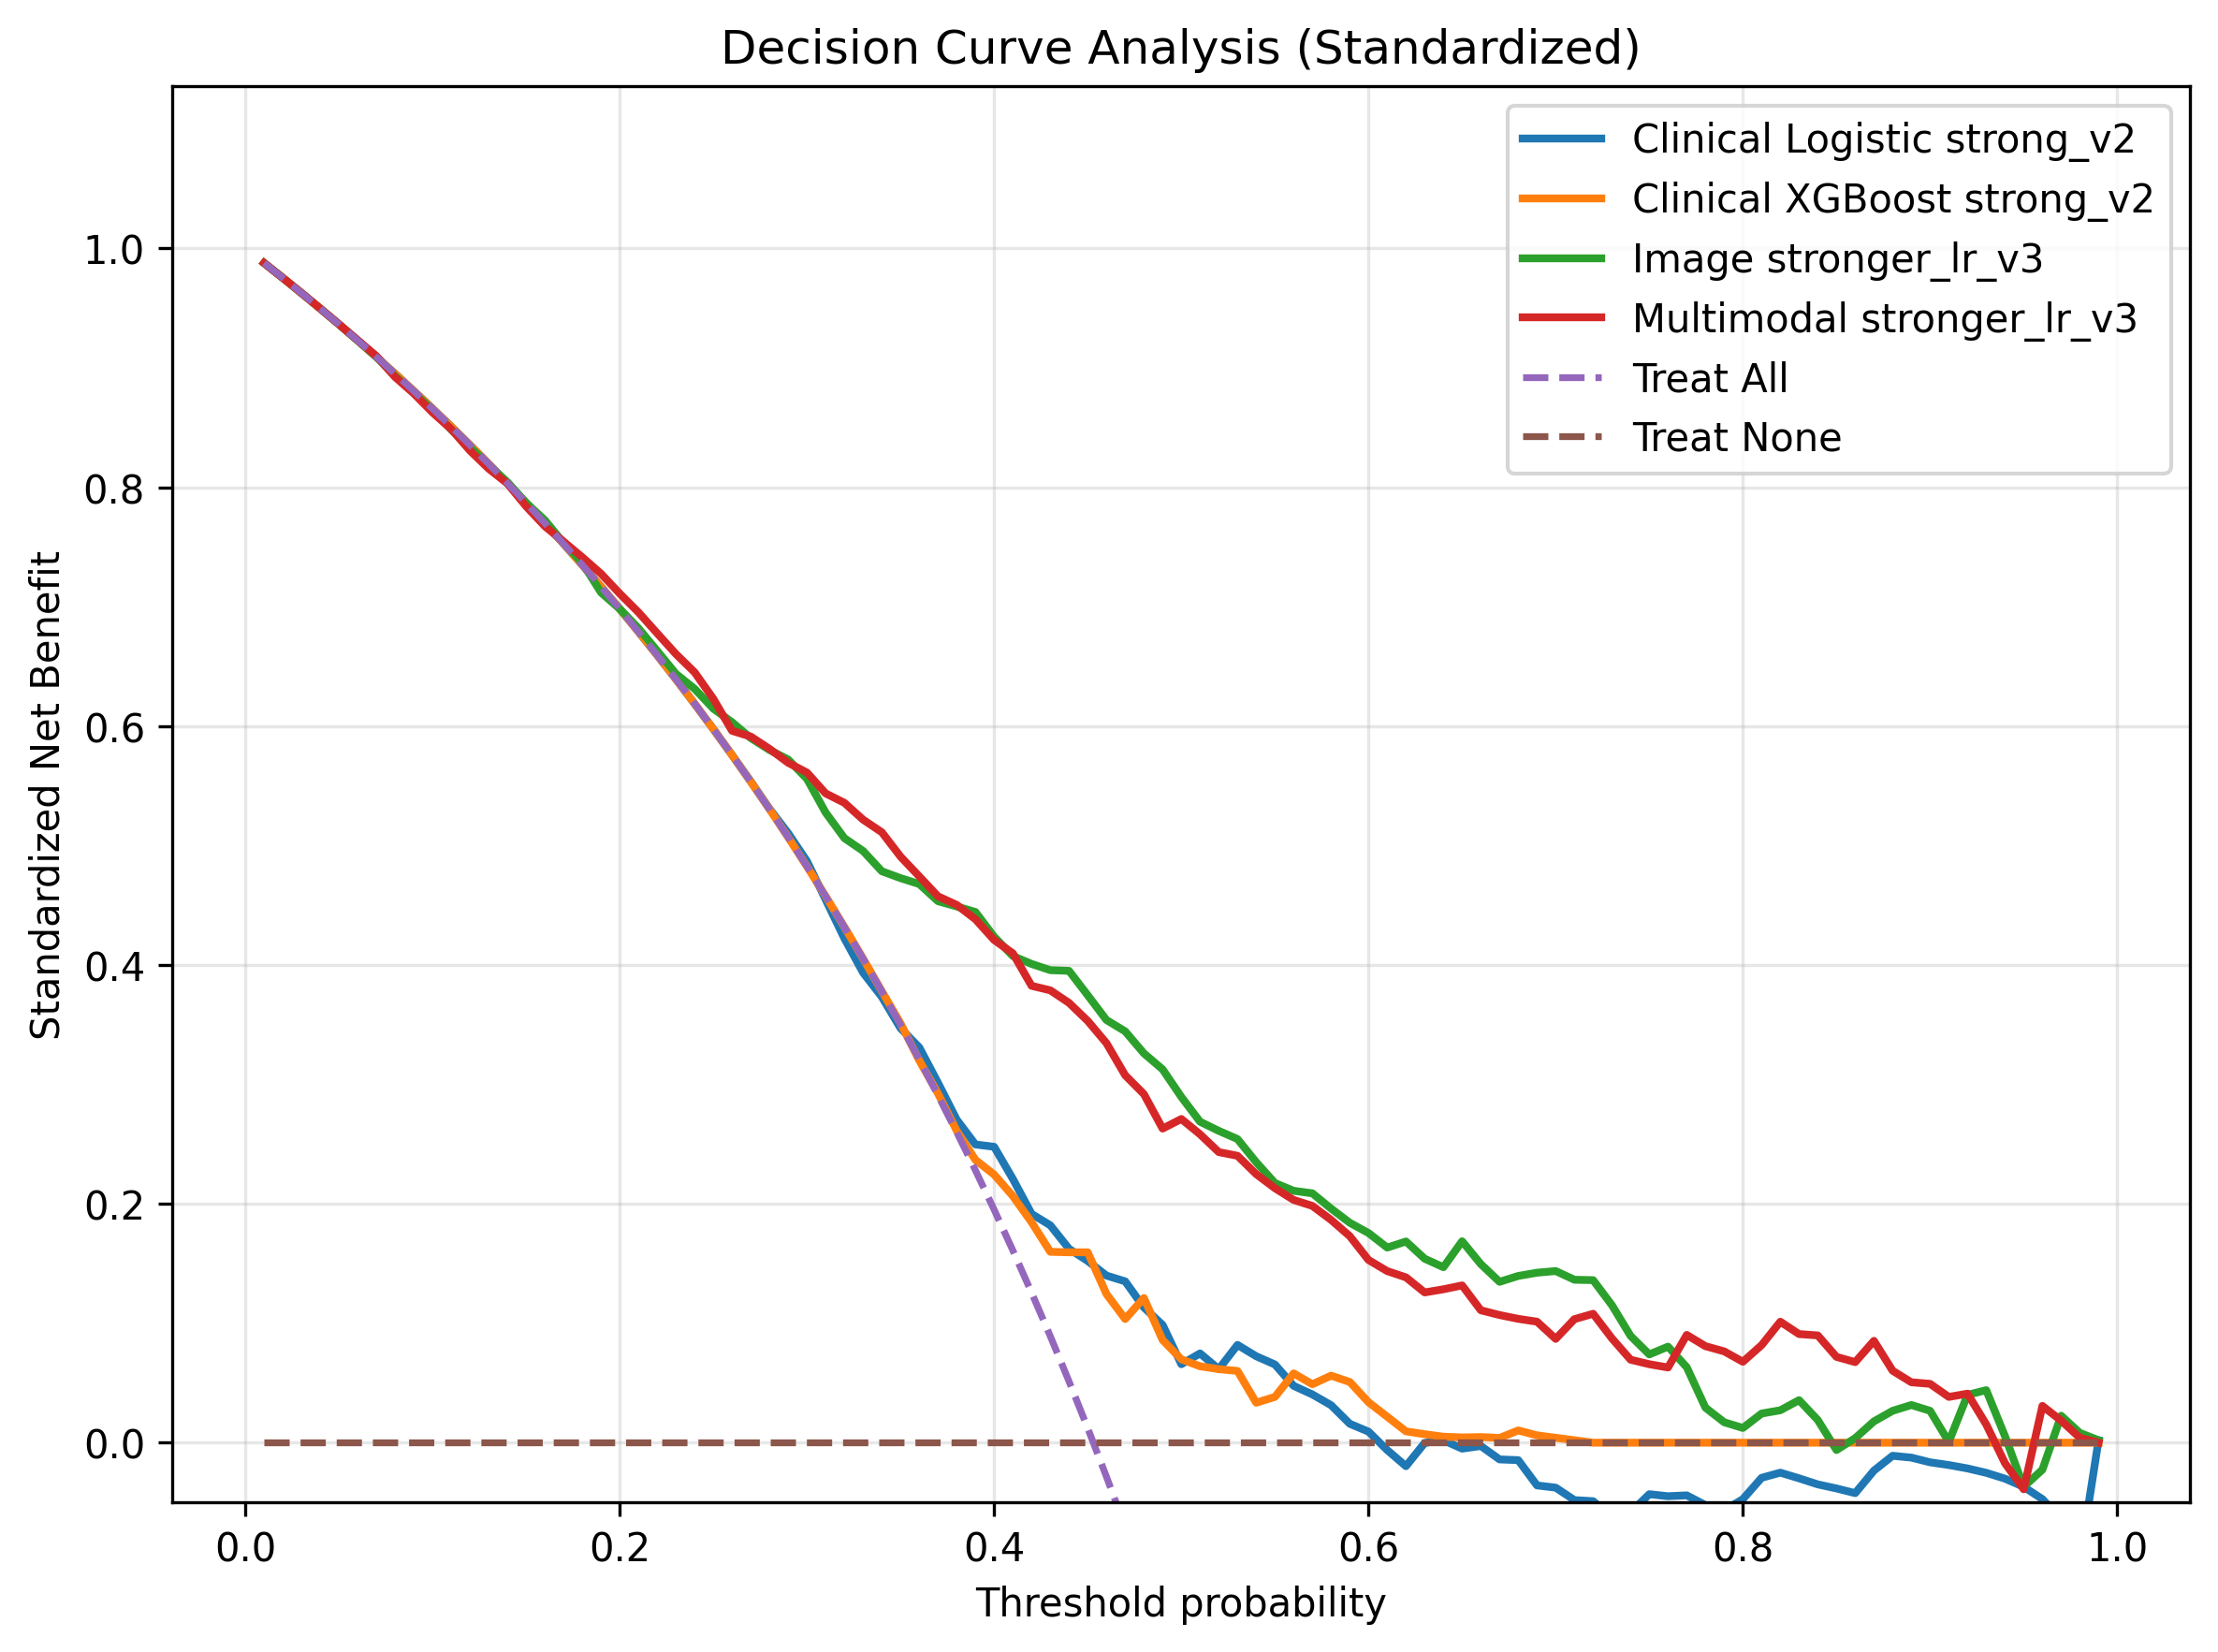
\includegraphics[width=0.8\textwidth]{images/decision_curve_standardized.png}
    \caption{Decision curve analysis for all models on the temporal test set. Both image-based models provide substantially greater net benefit than the clinical baselines, while the relative ordering of image-only and multimodal models depends on the operating threshold.}
    \label{fig:dca_all_models}
\end{figure}

Figure~\ref{fig:dca_all_models} shows that both image-based models provide substantially greater net benefit than the clinical baselines across the evaluated thresholds. The relative ordering of the image-only and multimodal models is threshold-dependent: the image model is higher at some thresholds, whereas the multimodal model is slightly higher at others. This pattern is consistent with the broader finding that multimodal fusion remains competitive but does not establish a clear overall advantage over the image-only baseline.

At a threshold of 0.5, net benefit values were approximately 0.030 (clinical logistic), 0.032 (clinical XGBoost), 0.131 (image), and 0.123 (multimodal). Full curves and tabulated results are available in the evaluation outputs.

Unlike AUROC or AUPRC, decision curve analysis translates predictive performance into a threshold-dependent utility perspective. In the present context, the DCA results reinforce two points. First, both deep learning models are substantially more useful than the triage-only baselines when decisions are made using a thresholded risk score. Second, the practical difference between image-only and multimodal systems depends on the selected threshold, rather than supporting a universal winner across all operating conditions.

\section{Qualitative Analysis}

To complement quantitative evaluation, qualitative analysis was performed using gradient-based class activation mapping (Grad-CAM) applied to representative predictions from the image model. This method highlights spatial regions that contribute most strongly to model predictions and serves as a qualitative diagnostic rather than a standalone validation method.

\begin{figure}[htbp]
    \centering

    \begin{minipage}{0.48\textwidth}
        \centering
        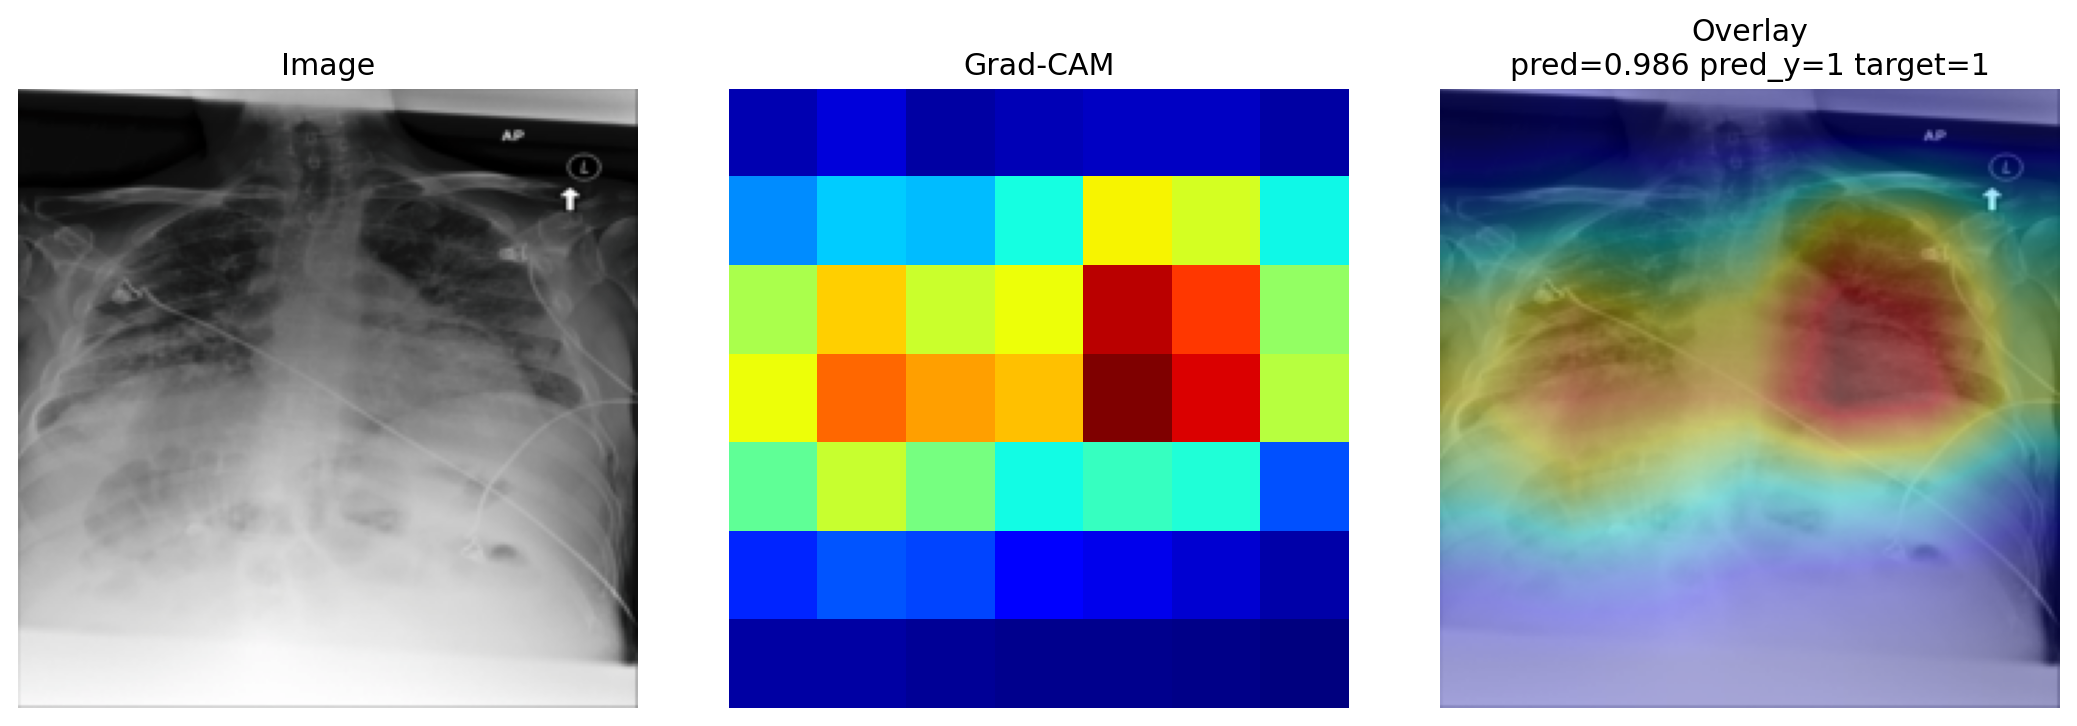
\includegraphics[width=\textwidth]{images/gradcam_tp1.png}
        \vspace{2pt}
        \small (a) True positive. Activation focuses on lower lung regions consistent with pneumonia.
    \end{minipage}
    \hfill
    \begin{minipage}{0.48\textwidth}
        \centering
        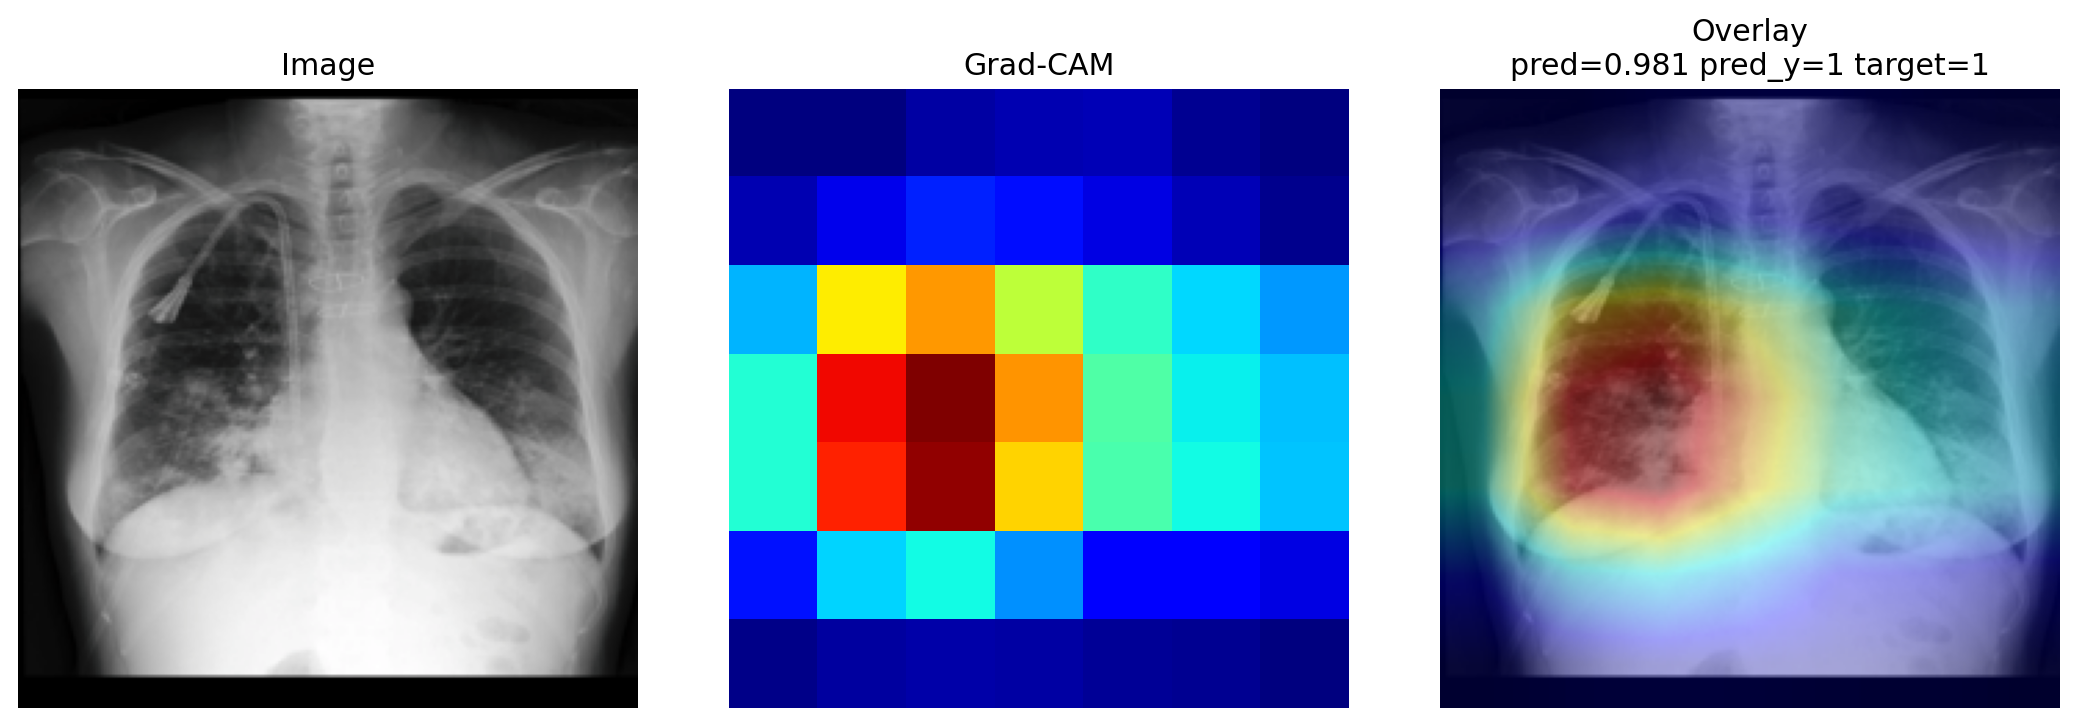
\includegraphics[width=\textwidth]{images/gradcam_tp2.png}
        \vspace{2pt}
        \small (b) True positive. Diffuse activation aligns with radiographic abnormalities.
    \end{minipage}

    \vspace{6pt}

    \begin{minipage}{0.48\textwidth}
        \centering
        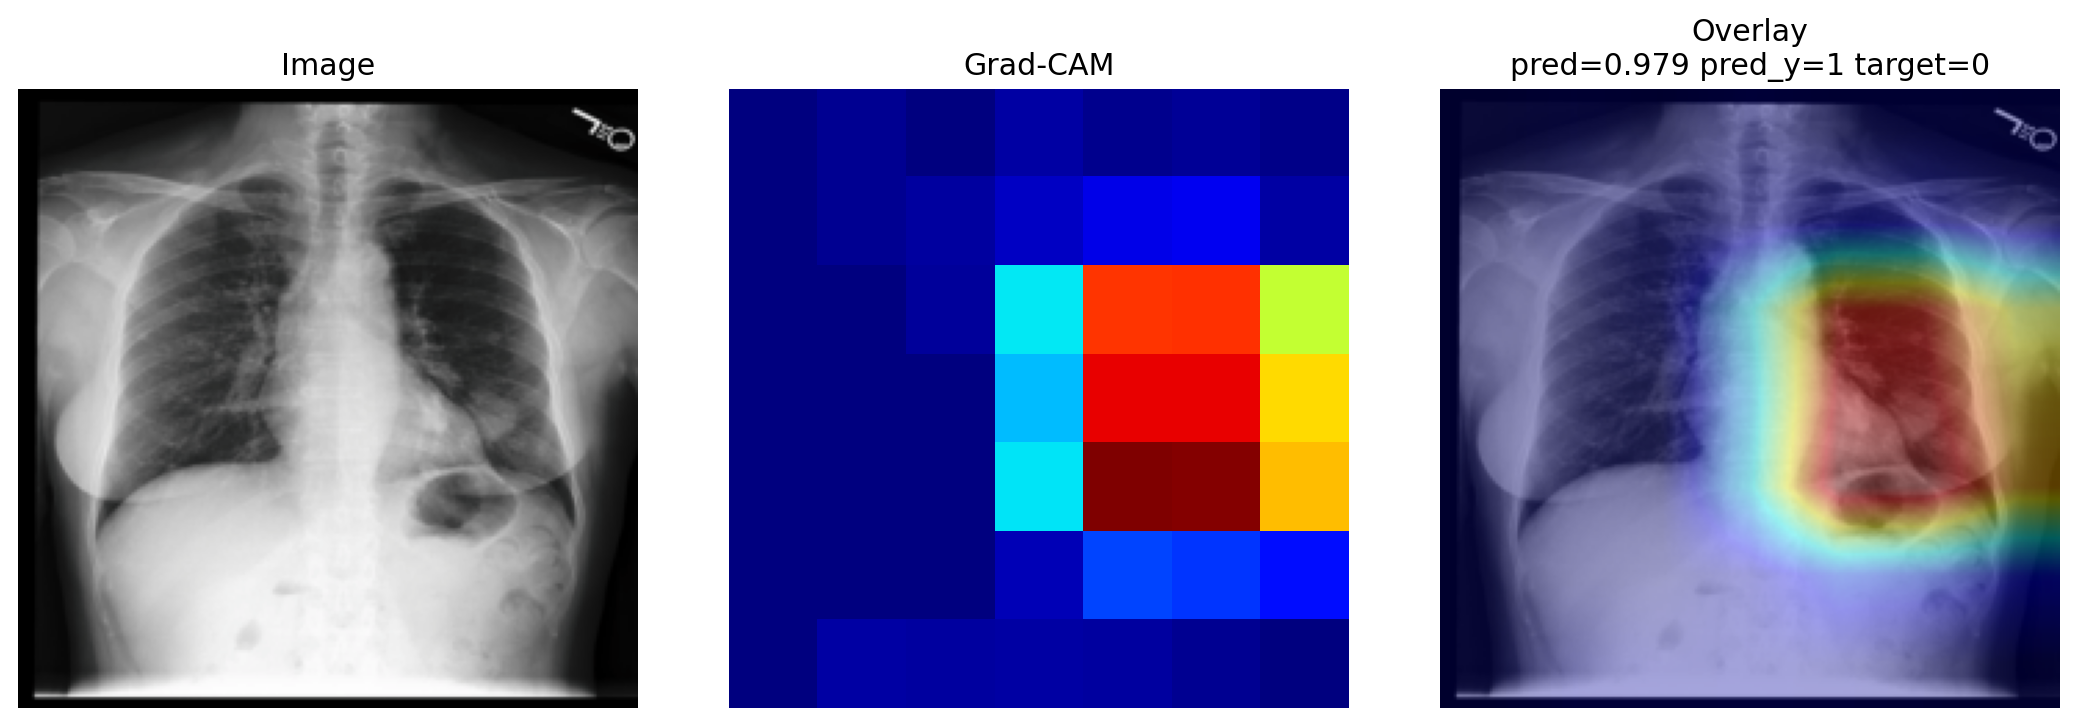
\includegraphics[width=\textwidth]{images/gradcam_fp.png}
        \vspace{2pt}
        \small (c) False positive. Attention is placed on non-pathological or non-specific abnormal structures.
    \end{minipage}
    \hfill
    \begin{minipage}{0.48\textwidth}
        \centering
        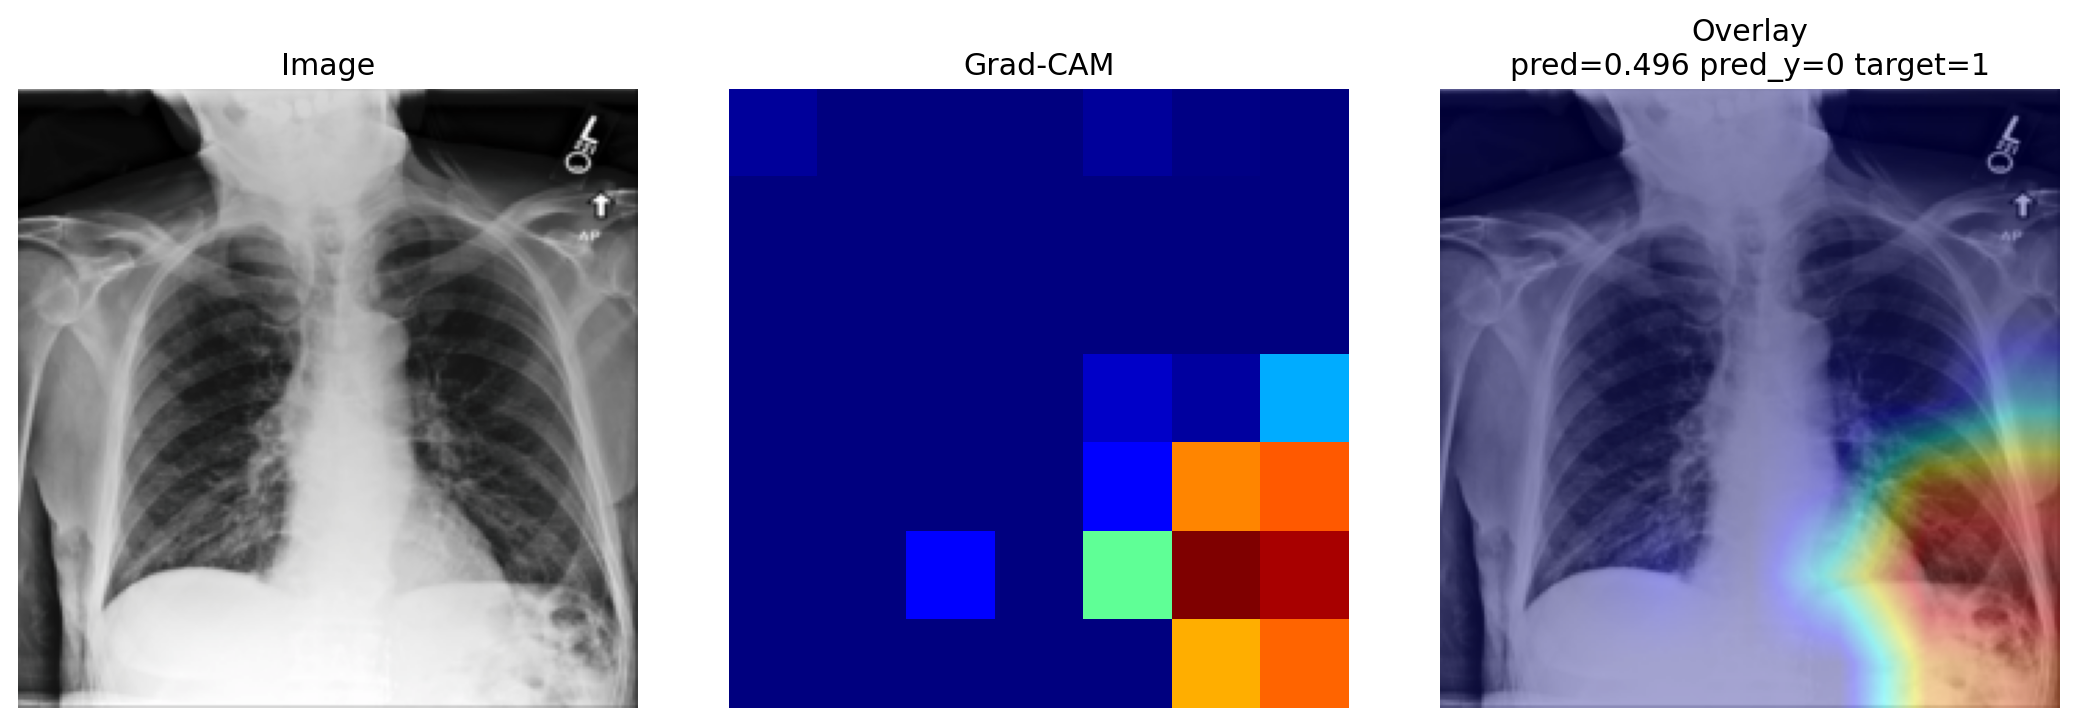
\includegraphics[width=\textwidth]{images/gradcam_fn.png}
        \vspace{2pt}
        \small (d) False negative. Weak activation over subtle or diffuse pathological regions.
    \end{minipage}

    \caption{Grad-CAM visualizations for representative cases from the image model. Heatmaps indicate regions contributing most strongly to predictions. Correct predictions align with plausible lung regions, while errors highlight sensitivity to confounders and missed subtle findings.}
    \label{fig:gradcam_cases}
\end{figure}

In correctly classified cases, the model attends to lung fields and regions consistent with pneumonia. False positives suggest sensitivity to confounding or non-specific visual patterns, while false negatives indicate difficulty in detecting subtle or diffuse abnormalities.

These qualitative examples do not serve as proof of general behavior by themselves, but they provide useful explanatory context for the quantitative results. In particular, the Grad-CAM cases suggest that correct predictions tend to arise when radiographic abnormalities are sufficiently localized or visually salient, whereas errors occur in settings where the visual evidence is weak, distributed, or confounded by other thoracic structures. This interpretation is consistent with the idea that the image model is strong when pneumonia presents with relatively clear radiographic correlates, but less reliable in ambiguous cases.

\section{Hard-Negative Analysis}

A stratified analysis based on CheXpert abnormality labels yielded 686 studies after restricting evaluation to rows with available abnormality-label information. This subset contained 392 pneumonia-positive studies, 132 normal negatives, and 162 abnormal negatives without pneumonia. For pneumonia versus normal negatives, AUROC was 0.769 for the image model and 0.755 for the multimodal model, with AUPRC values of 0.914 and 0.906, respectively. For pneumonia versus abnormal negatives, AUROC decreased to 0.632 for the image model and 0.599 for the multimodal model, with AUPRC values of 0.810 and 0.792. The corresponding AUROC differences between abnormal-negative and normal-negative subsets were approximately $-0.137$ for the image model and $-0.156$ for the multimodal model, with similar reductions observed for AUPRC.

This analysis is one of the most informative secondary results in the thesis. It shows that the apparent difficulty of the task depends strongly on how the negative class is defined. When negative cases are relatively normal, both image-based models separate them from pneumonia more effectively. When the negative class is restricted to other abnormal studies, discrimination falls substantially. This suggests that the true challenge is not simply to distinguish pneumonia from normal radiographs, but to distinguish pneumonia from other radiographic abnormalities with partially overlapping visual patterns.

The hard-negative analysis also provides a useful interpretation for both the Grad-CAM failure cases and the limited multimodal gain. If the dominant difficulty lies in differentiating among multiple abnormal thoracic presentations, then triage variables alone may not be sufficiently specific to resolve that ambiguity. In this setting, it is plausible that the image representation remains the dominant source of useful information, while the structured clinical features add limited incremental signal. Notably, the drop in AUROC between normal-negative and abnormal-negative subsets is somewhat larger for the multimodal model than for the image-only model, suggesting that fusion does not resolve this ambiguity in the present formulation.
\chapter{Discussion}

\section{Summary of Findings}

The empirical results support three main observations. First, the image-only DenseNet121 model achieves the highest discrimination and threshold-based performance on the held-out temporal test set, while the clinical models are substantially weaker on AUROC and AUPRC. This indicates that, within the present cohort and label definition, chest radiographs contain substantially more task-relevant information for radiographic pneumonia prediction than the selected triage variables alone.

Second, early multimodal fusion does not improve over the image-only baseline. Although the multimodal model remains competitive in absolute terms and clearly exceeds the clinical-only baselines, point estimates favor the image model, and paired bootstrap intervals for multimodal-minus-image differences include zero for both AUROC and AUPRC. The fraction of patient-level bootstrap resamples favoring the multimodal model is also low. Taken together, these results do not support the claim that multimodal fusion provides a reliable performance advantage in the present setup.

Third, the auxiliary analyses show that model behavior is more nuanced than a single discrimination metric suggests. Calibration differs from discrimination, with the multimodal model exhibiting somewhat better-calibrated probabilities than the image-only model under fixed-bin calibration metrics despite weaker ranking performance. Decision curve analysis places both deep models above the clinical baselines, but again does not establish a clear multimodal advantage across thresholds. Finally, performance varies substantially across negative-case subtypes, with marked degradation when the negative class is restricted to other abnormal radiographs rather than relatively normal studies. This indicates that task difficulty depends strongly on the structure of the comparator group.

Taken together, these findings support a central conclusion of the thesis: under strict temporal constraints and a radiograph-centered label definition, a strong image model dominates predictive performance, while multimodal fusion with triage variables does not provide a consistent additional benefit.

\section{Interpretation of Multimodal Performance}

The absence of a multimodal advantage is one of the most important results of this thesis. While multimodal learning is often assumed to be beneficial, the present findings suggest that such benefit is conditional rather than automatic. Several plausible factors may explain why the multimodal model does not improve on the image-only baseline, although the current experiments cannot establish any of them as definitive causal mechanisms.

A first factor is the limited incremental value of the available tabular data. The structured clinical branch is restricted to triage variables available at or before the imaging time. These measurements encode patient state at presentation, but they are relatively coarse compared with the spatially rich information present in a chest radiograph. Once an image has already been observed by the model, triage variables may add only limited independent signal for the specific task of radiographic pneumonia prediction.

A second factor is redundancy between modalities. Acute respiratory illness can manifest simultaneously in both physiology and imaging. Tachypnea, low oxygen saturation, and elevated temperature may correlate with pneumonia, but they may also correlate with many other respiratory or systemic conditions. If these variables overlap strongly with information that is already implicitly represented in the radiograph embedding, then early fusion may add complexity without adding enough unique signal to improve discrimination.

A third factor is representation-level asymmetry between the two branches. In the implemented multimodal model, the image encoder produces a high-dimensional visual representation learned from multilabel pretraining and task-specific fine-tuning, whereas the structured branch is built from a relatively small set of triage variables. It is therefore plausible that the fused representation is dominated by the image pathway, with the clinical branch contributing only weakly or inconsistently. This does not mean the triage information is irrelevant in principle, but it does suggest that its incremental value may be limited under the present task formulation.

A fourth factor is architectural limitation. The implemented multimodal model uses a relatively simple early-fusion strategy: a DenseNet-derived image embedding is concatenated with a learned tabular representation and passed through a compact fusion head. This is a reasonable and interpretable design for a thesis, but it may not fully exploit complex cross-modal relationships. More expressive fusion mechanisms, alternative conditioning schemes, or deeper tabular encoders might behave differently. However, the thesis result remains meaningful even without such extensions: under the chosen and well-defined fusion design, no robust multimodal gain is observed.

A fifth factor is optimization difficulty. Multimodal systems are harder to train than unimodal ones because they require the coordinated optimization of multiple branches and a fusion mechanism. Even if the tabular modality contains some complementary signal, that signal may be difficult to exploit effectively without more careful architectural or optimization choices. In that sense, a negative result for early fusion does not imply that clinical information is irrelevant in principle; rather, it shows that its benefit is not guaranteed in the present formulation.

For a thesis, this finding is valuable precisely because it is honest and constrained. The result is not framed as a failure of multimodal learning in general, but as evidence that multimodal benefit must be demonstrated empirically within a carefully defined setting.

\section{Role of Temporal Constraints}

A defining methodological feature of this work is the explicit anchoring of prediction at the imaging time, with strict exclusion of features that may depend on post-imaging events. This decision is central to the scientific validity of the thesis. In medical machine learning, strong performance can be misleading when the feature set contains variables that are not genuinely available at prediction time. Such leakage may arise subtly, especially in multimodal pipelines that combine data sources recorded at different stages of the clinical workflow.

In the present study, triage inputs are aligned with a pre-result clinical state, and variables such as disposition are excluded due to their potential dependence on downstream decisions. Likewise, patient-level temporal splitting prevents the same patient from appearing across train and test in a way that would compromise the interpretation of generalization. Together, these decisions make the reported performance more conservative, but also more credible.

This point is important for interpreting the absolute metric values. A less restrictive pipeline could potentially yield higher AUROC or AUPRC by exploiting future information, repeated-patient structure, or downstream documentation artifacts. However, such gains would not reflect a clean solution to the intended prediction problem. The current setup instead prioritizes temporal validity over maximal feature inclusion, ensuring that reported performance corresponds to a well-defined clinical decision point.

From a thesis perspective, this design choice is a strength. Even if temporal rigor makes the problem harder and reduces the apparent payoff of multimodal fusion, it increases the trustworthiness of the conclusions. The thesis therefore emphasizes methodological validity rather than maximizing benchmark performance at all costs.

\section{Error Structure and Negative Definition}

The abnormal-negative analysis provides one of the clearest insights into the structure of the task. Stratification by CheXpert abnormality labels reveals a substantial decline in performance when negatives are restricted to studies with other radiographic abnormalities, compared with relatively normal negatives. This suggests that the main challenge is not simply to distinguish pneumonia from normal radiographs, but to distinguish pneumonia from other abnormal thoracic presentations that may share overlapping visual patterns.

This result helps explain why the image-only model, despite being the strongest overall, still exhibits substantial error. A model may appear to perform well when the negative class is dominated by relatively normal cases, but its effective task becomes much harder when non-pneumonia abnormalities are included. In such settings, the decision boundary must separate among multiple visually similar pathological states rather than between clearly healthy and clearly diseased images.

The negative-definition result also supports the qualitative findings from Grad-CAM. In the present project, the interpretability examples are generated from the image-only DenseNet121 model and are intended as descriptive diagnostics rather than causal explanations. False positives appear to arise in cases where the model responds to visually abnormal but non-pneumonic structures or patterns, whereas false negatives arise when the radiographic signal is subtle, diffuse, or ambiguous. These observations are consistent with the idea that the learned image representation is highly sensitive to overt abnormality, but not perfectly specific for pneumonia as a distinct radiographic concept.

More broadly, this analysis illustrates that label design and evaluation cohort construction are inseparable from model interpretation. A binary pneumonia label derived from report structure is necessarily embedded within a broader ontology of thoracic findings. As a consequence, reported binary performance metrics must be interpreted with caution: they reflect not only model quality, but also the composition of positive and negative cases.

\section{Task Ambiguity as a Central Finding}

One of the most important conceptual findings of the thesis is that radiographic pneumonia detection, as implemented here, is an inherently ambiguous problem rather than a clean binary discrimination task. This ambiguity arises from at least three interacting sources.

The first source is label ambiguity. The primary target is derived from CheXpert report labels and therefore reflects a report-based radiographic proxy for pneumonia rather than a definitive etiologic diagnosis. The \texttt{u\_ignore} policy reduces ambiguity by excluding uncertain annotations, but it does not eliminate residual label noise or the broader mismatch between radiographic appearance and underlying disease mechanism. Even a carefully trained model is therefore learning against an imperfect target.

The second source is radiographic overlap. Pneumonia shares visual characteristics with other thoracic abnormalities, including pleural effusion, pulmonary edema, and non-specific parenchymal opacity. The hard-negative analysis makes this explicit: both image-only and multimodal performance decline substantially when the comparison class is restricted to other abnormal studies. This indicates that the difficulty of the task is not accidental or limited to a few edge cases, but is built into the visual structure of the problem itself.

The third source is limited specificity in the structured modality. Triage-at-\(t_0\) variables may reflect the presence of acute illness, but they are not highly specific for radiographic pneumonia. Fever, tachypnea, hypoxemia, and abnormal blood pressure can accompany many other conditions. As a result, adding these variables to the image pathway does not necessarily resolve the ambiguity created by overlapping radiographic findings.

Taken together, these three sources suggest that the key result of the thesis is not merely that image-only performance exceeds multimodal performance, but that the benchmark itself encodes an ambiguity-rich discrimination problem. Under this formulation, the image model is not failing because it is weak; rather, it is operating near the limits imposed by overlapping radiographic patterns, imperfect supervision, and limited complementary structured information. This framing helps explain both the hard-negative findings and the absence of a robust multimodal advantage.

\section{Calibration and Clinical Relevance}

Calibration metrics show that the deep models achieve lower Brier scores than the clinical baselines, indicating improved average agreement between predicted probabilities and observed outcomes. However, expected calibration error does not follow the same ranking as discrimination, with the image model exhibiting a higher point ECE than the multimodal model despite superior AUROC. Maximum calibration error also varies across models. These findings reinforce that discrimination and calibration measure different properties of predictive systems.

This distinction is especially relevant in clinical settings. A model with stronger ranking performance may still produce probabilities that are poorly aligned with empirical event frequencies, which could be problematic if outputs are interpreted as risk estimates rather than merely as ranking scores. The present results suggest that the multimodal model, despite weaker discrimination than the image-only system, may produce somewhat better-calibrated probabilities under the fixed-bin calibration metrics used here.

At the same time, lower ECE for the multimodal model does not by itself override the stronger AUROC and AUPRC of the image model. The preferred metric depends on the intended use. In ranking-oriented workflows, stronger discrimination may be more valuable; in settings where predicted probabilities are communicated directly or interpreted as risk estimates, calibration quality becomes more important. The thesis therefore does not claim a single universally superior model across all possible use cases, but rather shows that model preference depends on which property of predictive performance is prioritized.

Decision curve analysis offers a complementary view by asking whether a model would improve threshold-based decision making relative to simpler alternatives. In this study, both deep models achieve substantially higher net benefit than the clinical baselines across the evaluated thresholds. The relative ordering of the image-only and multimodal models is threshold-dependent, which is consistent with the broader finding that multimodal fusion is competitive but not clearly superior overall. This result is also consistent with the fixed-threshold main table: multimodal slightly improves precision at 0.5, whereas image retains better overall ranking and recall.

At the same time, these decision-oriented results should not be overinterpreted. Net benefit depends on assumptions about intervention trade-offs and threshold selection that are not estimated directly from this dataset. Thus, the DCA findings should be read as supportive evidence of relative utility rather than as a claim of immediate clinical readiness. More broadly, they reinforce the value of evaluating models beyond AUROC alone, especially when deployment decisions would depend on calibrated probabilities or threshold-based actions.

\section{Limitations}

Several limitations should be acknowledged. First, the study relies on CheXpert-derived pneumonia labels under a policy that excludes uncertain annotations. This reduces ambiguity relative to treating uncertain labels as negatives, but it may also remove challenging cases and does not eliminate residual label noise. The target remains a report-derived radiographic formulation of pneumonia rather than a definitive microbiological or clinically adjudicated diagnosis.

Second, all experiments are conducted on a single MIMIC-derived cohort. Although the dataset is large and widely used, it does not establish generalization to other hospitals, patient populations, imaging protocols, or clinical workflows. No external validation is performed in the present thesis, and therefore the conclusions should be understood as internally valid within the studied setting rather than universally generalizable.

Third, the multimodal analysis is intentionally restricted to triage features. This is methodologically consistent with the thesis emphasis on strict feature timing, but it also limits the breadth of the structured clinical modality. Additional sources such as laboratory data, medication history, or longitudinal context are not included in the primary comparison. Laboratory features were explored in the broader project, but their low coverage makes them more appropriate as a sensitivity analysis than as a core thesis modality.

Fourth, the architecture search space is limited. The multimodal model provides a clear and interpretable early-fusion baseline, but it is not an exhaustive search over possible multimodal designs. Similarly, the image model is strong but not necessarily optimal among all possible radiograph architectures. The goal of the thesis is rigorous comparative evaluation under controlled conditions, not maximal engineering optimization.

Fifth, most threshold-based summary metrics in the main results table are reported at a fixed probability threshold of 0.5. This is a standard reference point, but it should not be interpreted as an optimized clinical operating threshold. Different deployment scenarios could favor different thresholds and therefore different trade-offs between precision, recall, and net benefit.

Sixth, no post hoc recalibration comparison, such as temperature scaling or isotonic regression, is included in the primary analysis. As a result, the calibration results should be interpreted as properties of the raw model outputs rather than as the best achievable calibrated versions of these models.

Seventh, the abnormal-negative analysis is restricted to the subset of cases with available CheXpert abnormality annotations and should therefore be interpreted as a secondary descriptive analysis rather than as a separate benchmark. Even so, its consistency with the qualitative findings strengthens its interpretive value.

\section{Future Work}

Several directions for future work follow naturally from the present results. A first direction is to evaluate alternative target formulations, especially clinically actionable pneumonia definitions that differ from the current radiographic label. This would directly address the label ambiguity highlighted in the present study and could change the relative value of structured clinical inputs.

A second direction is to extend the multimodal modelling strategy itself. Richer fusion mechanisms, deeper tabular encoders, or alternative training schedules could be used to test whether the absence of multimodal gain is architectural rather than informational. In parallel, systematic ablations could be performed to identify which subsets of clinical variables contribute most, if at all, once radiographic information is available.

A third direction is to incorporate additional structured modalities under carefully defined timing rules. Laboratory data are an obvious candidate, but their usefulness depends on availability, timing, and missingness. In the current project, laboratory coverage is too limited for a fair primary comparison, but it remains a reasonable sensitivity-analysis direction and a possible extension in future datasets or expanded cohorts.

Finally, external and multi-site validation would be required to assess robustness and generalizability beyond the current MIMIC-based environment. Such validation is outside the scope of the thesis, but it represents an essential step for any future attempt to translate the conclusions into broader clinical use.
\chapter{Conclusion}

This thesis investigated binary radiographic pneumonia detection in an emergency department--linked cohort derived from MIMIC-CXR-JPG and MIMIC-IV-ED. The study compared triage-only clinical baselines, an image-only DenseNet121 classifier, and an early-fusion multimodal model combining triage features with chest radiographs. A central design principle was the explicit anchoring of prediction at the time of imaging, with all inputs restricted to information available at or before that moment. This constraint ensured that the task corresponds to a well-defined and clinically meaningful decision point and that reported results are aligned with a realistic deployment-time information setting.

On a shared patient-level temporal test partition, the image-only model achieved the strongest overall performance across both discrimination and threshold-based metrics. In particular, the image-only model achieved AUROC 0.746 and AUPRC 0.724, compared with 0.736 and 0.714 for the multimodal model. Paired patient-level bootstrap comparisons of multimodal minus image produced uncertainty intervals for both AUROC and AUPRC that included zero, indicating no reliable advantage from fusion in this setting. Both deep learning models substantially outperformed the clinical baselines, demonstrating that chest radiographs provide significantly stronger predictive signal for this task than the selected triage variables.

Beyond these primary results, the thesis provides additional insight into the structure of the problem itself. Performance was shown to depend strongly on the composition of the negative class, with a marked decrease when distinguishing pneumonia from other abnormal radiographs compared with relatively normal cases. These subgroup effects indicate that the benchmark is intrinsically ambiguous: separating pneumonia from other abnormal thoracic findings is substantially harder than separating pneumonia from relatively normal studies. Calibration analysis further demonstrated that discrimination and probabilistic reliability are distinct properties, with the multimodal model exhibiting somewhat improved calibration under fixed-bin metrics despite lower ranking performance. Decision curve analysis confirmed that both image-based models provide higher utility than the clinical baselines across a range of thresholds, while again showing no clear overall advantage of multimodal fusion over the image-only system.

Taken together, these findings challenge the assumption that multimodal integration is inherently beneficial. In the present setting, where tabular inputs are limited to pre-imaging triage data and strict temporal constraints are enforced, a strong image model captures most of the useful predictive signal. Multimodal fusion, at least in its current form, introduces additional complexity without yielding a consistent performance gain. This result does not imply that multimodal learning is ineffective in general, but rather that its value depends critically on the nature, timing, and complementarity of the available modalities.

More broadly, this work highlights the importance of rigorous problem formulation and evaluation design in medical machine learning. Explicit temporal alignment, leakage-aware feature selection, and patient-level evaluation are not merely implementation details; they fundamentally shape both the difficulty of the task and the validity of the conclusions. Under the strict temporal constraints used here, methodological validity determined which conclusions could be trusted: robust image-only superiority over clinical baselines, but no reliable multimodal gain.

In summary, this thesis demonstrates that careful control of data, time, and evaluation is as important as model architecture in determining the outcome of medical AI systems. The results emphasize that strong unimodal baselines should be established before claiming multimodal benefit, that pneumonia detection in this setting is intrinsically ambiguity-rich, and that empirical validation under realistic constraints is essential for drawing reliable conclusions. These findings should be understood as internal to the present MIMIC-based benchmark, but they provide a strong foundation for future work on alternative targets, richer structured inputs, and broader external validation.

\appendix
\chapter{Feature Dictionary}

This appendix documents the structured variables used in the primary triage-based clinical and multimodal models. The active feature policy is intentionally restricted to variables that are available at or before the imaging time ($t_0$), in order to preserve temporal validity and reduce the risk of information leakage from downstream clinical decisions.

The primary structured feature set is derived from emergency department triage data linked to the chest radiograph cohort. It consists of four groups of variables: numeric physiological variables, categorical context variables, explicit missingness indicators for numeric fields, and binary view-position flags inherited from the imaging pipeline. The same core triage feature set is used in the headline clinical logistic regression model, the headline clinical XGBoost model, and the structured branch of the headline multimodal model.

Feature construction is implemented through the triage linkage and feature-building pipeline, primarily in \texttt{src/data/link\_cxr\_to\_triage.py}, \texttt{src/data/build\_triage\_features.py}, and \texttt{src/data/build\_triage\_model\_table.py}. The active feature policy is also described in \texttt{docs/triage\_feature\_policy.md}. Missingness counts are recorded in artifact reports, but precomputed missingness percentages were not found as direct stored outputs in the repository. Likewise, units are only partially explicit in code comments; beyond temperature, exact units are generally not encoded directly in the stored feature tables and are therefore treated here as \emph{not explicitly documented in code} unless otherwise stated.

\section{Included Features}

The features included in the primary triage-based models are grouped as follows.

\subsection*{Numeric Variables}
\begin{itemize}
    \item \texttt{temperature}
    \item \texttt{heartrate}
    \item \texttt{resprate}
    \item \texttt{o2sat}
    \item \texttt{sbp}
    \item \texttt{dbp}
    \item \texttt{pain}
    \item \texttt{acuity}
\end{itemize}

\subsection*{Missingness Indicators}
\begin{itemize}
    \item \texttt{temperature\_missing}
    \item \texttt{heartrate\_missing}
    \item \texttt{resprate\_missing}
    \item \texttt{o2sat\_missing}
    \item \texttt{sbp\_missing}
    \item \texttt{dbp\_missing}
    \item \texttt{pain\_missing}
    \item \texttt{acuity\_missing}
\end{itemize}

\subsection*{Binary Flags}
\begin{itemize}
    \item \texttt{is\_pa}
    \item \texttt{is\_ap}
\end{itemize}

\subsection*{Categorical Variables}
\begin{itemize}
    \item \texttt{gender}
    \item \texttt{race}
    \item \texttt{arrival\_transport}
\end{itemize}

\section{Preprocessing and Feature Policy}

Numeric variables are coerced to numeric type, with implausible values clipped for several vital-sign fields during triage feature construction. In the logistic regression and multimodal pipelines, these variables are subsequently median-imputed and standardized. In the XGBoost pipeline, numeric values are used after coercion without an explicit scaling stage. Categorical variables are normalized to strings, trimmed, and mapped to \texttt{UNKNOWN} when missing or empty. In the logistic regression and multimodal pipelines, they are imputed with a constant \texttt{UNKNOWN} token and one-hot encoded; in XGBoost, they are cast to categorical type for native handling. Missingness indicators are explicitly created during feature construction and then filled to one when absent during model preparation.

Several plausibility filters are explicitly implemented in \texttt{src/data/build\_triage\_features.py}. Temperature is clipped to the range 95.0 to 105.8, with a code comment indicating Fahrenheit. Heart rate is clipped to 30--220, respiratory rate to 5--60, oxygen saturation to 50--100, systolic blood pressure to 60--250, and diastolic blood pressure to 30--150. No explicit clipping is implemented for \texttt{pain} or \texttt{acuity} in the same feature-construction stage.

The two binary flags, \texttt{is\_pa} and \texttt{is\_ap}, are not native triage variables but propagated imaging-view indicators inherited from the radiograph selection pipeline. They are included as structured inputs in all primary model families because view position may affect radiographic appearance and therefore influence prediction behavior.

\section{Excluded or Leakage-Sensitive Fields}

Two fields are explicitly notable in the repository but are not part of the active primary baseline feature set:

\begin{itemize}
    \item \texttt{disposition}: explicitly removed or marked as leakage-prone in both documentation and feature-building code because it may reflect downstream post-\(t_0\) clinical decisions.
    \item \texttt{chiefcomplaint}: present at intermediate stages of feature building, but explicitly excluded from the baseline clinical and multimodal models.
\end{itemize}

This exclusion policy is important for the thesis because it demonstrates that the structured branch was designed around time-safe variables rather than convenience or maximal feature inclusion.

\section{Detailed Feature Table}

\renewcommand{\arraystretch}{1.15}
\small
\begin{longtable}{p{2.6cm} p{2.2cm} p{2.3cm} p{6.8cm}}
\toprule
\textbf{Feature} & \textbf{Type} & \textbf{Used In} & \textbf{Preprocessing / Notes} \\
\midrule
\endfirsthead

\toprule
\textbf{Feature} & \textbf{Type} & \textbf{Used In} & \textbf{Preprocessing / Notes} \\
\midrule
\endhead

\texttt{temperature} & Numeric & All primary models & Numeric coercion; clipped to 95.0--105.8; median imputation + standardization in logistic/multimodal; raw coerced numeric in XGBoost. Code comment indicates Fahrenheit. \\
\texttt{heartrate} & Numeric & All primary models & Numeric coercion; clipped to 30--220; median imputation + standardization in logistic/multimodal; raw coerced numeric in XGBoost. \\
\texttt{resprate} & Numeric & All primary models & Numeric coercion; clipped to 5--60; median imputation + standardization in logistic/multimodal; raw coerced numeric in XGBoost. \\
\texttt{o2sat} & Numeric & All primary models & Numeric coercion; clipped to 50--100; median imputation + standardization in logistic/multimodal; raw coerced numeric in XGBoost. \\
\texttt{sbp} & Numeric & All primary models & Numeric coercion; clipped to 60--250; median imputation + standardization in logistic/multimodal; raw coerced numeric in XGBoost. \\
\texttt{dbp} & Numeric & All primary models & Numeric coercion; clipped to 30--150; median imputation + standardization in logistic/multimodal; raw coerced numeric in XGBoost. \\
\texttt{pain} & Numeric & All primary models & Numeric coercion; no explicit clipping found; median imputation + standardization in logistic/multimodal; raw coerced numeric in XGBoost. \\
\texttt{acuity} & Numeric & All primary models & Numeric coercion; no explicit clipping found; median imputation + standardization in logistic/multimodal; raw coerced numeric in XGBoost. \\
\texttt{temperature\_missing} & Missingness indicator & All primary models & Derived as missingness flag; filled to 1 and cast to integer in model preparation. \\
\texttt{heartrate\_missing} & Missingness indicator & All primary models & Derived as missingness flag; filled to 1 and cast to integer in model preparation. \\
\texttt{resprate\_missing} & Missingness indicator & All primary models & Derived as missingness flag; filled to 1 and cast to integer in model preparation. \\
\texttt{o2sat\_missing} & Missingness indicator & All primary models & Derived as missingness flag; filled to 1 and cast to integer in model preparation. \\
\texttt{sbp\_missing} & Missingness indicator & All primary models & Derived as missingness flag; filled to 1 and cast to integer in model preparation. \\
\texttt{dbp\_missing} & Missingness indicator & All primary models & Derived as missingness flag; filled to 1 and cast to integer in model preparation. \\
\texttt{pain\_missing} & Missingness indicator & All primary models & Derived as missingness flag; filled to 1 and cast to integer in model preparation. \\
\texttt{acuity\_missing} & Missingness indicator & All primary models & Derived as missingness flag; filled to 1 and cast to integer in model preparation. \\
\texttt{is\_pa} & Binary flag & All primary models & Propagated imaging-view flag from the frontal-image selection pipeline; filled to 0 when absent; treated as numeric input. \\
\texttt{is\_ap} & Binary flag & All primary models & Propagated imaging-view flag from the frontal-image selection pipeline; filled to 0 when absent; treated as numeric input. \\
\texttt{gender} & Categorical & All primary models & String normalization; missing or empty mapped to \texttt{UNKNOWN}; one-hot encoded in logistic/multimodal; categorical dtype in XGBoost. \\
\texttt{race} & Categorical & All primary models & String normalization; missing or empty mapped to \texttt{UNKNOWN}; one-hot encoded in logistic/multimodal; categorical dtype in XGBoost. \\
\texttt{arrival\_transport} & Categorical & All primary models & String normalization; missing or empty mapped to \texttt{UNKNOWN}; one-hot encoded in logistic/multimodal; categorical dtype in XGBoost. \\
\bottomrule
\end{longtable}
\normalsize

\section{Feature Provenance and Time-Safety Checks}

The primary feature set documented here is identical across the clinical logistic regression baseline, the clinical XGBoost baseline, and the structured branch of the multimodal model. This consistency is important because it ensures that performance differences among those systems arise from model family and modality interactions rather than from changes in the structured input definition.

Feature provenance and time-safety are supported by the following implementation components:

\begin{itemize}
    \item \texttt{src/data/build\_triage\_features.py}: constructs cleaned triage variables, plausibility filtering, and missingness indicators.
    \item \texttt{src/data/build\_triage\_model\_table.py}: defines the structured model table used by downstream training scripts.
    \item \texttt{docs/triage\_feature\_policy.md}: records the intended time-safe baseline policy and leakage-sensitive exclusions.
\end{itemize}

No precomputed feature-level missingness percentages were found as direct stored values in the repository, although missingness counts are available in artifact reports. Similarly, except for the temperature code comment, units are generally not stored as explicit metadata in the feature tables. These omissions do not affect the training pipeline itself, but they do limit the level of direct variable metadata available for reporting.

\section{Artifact References}

Relevant artifact and source locations include:

\begin{itemize}
    \item \texttt{src/models/clinical\_baseline.py}
    \item \texttt{src/models/clinical\_xgb.py}
    \item \texttt{src/training/train\_multimodal\_pneumonia.py}
    \item \texttt{src/data/build\_triage\_features.py}
    \item \texttt{src/data/build\_triage\_model\_table.py}
    \item \texttt{docs/triage\_feature\_policy.md}
    \item \texttt{artifacts/manifests/cxr\_ed\_triage\_features\_report.json}
    \item \texttt{artifacts/manifests/cxr\_ed\_triage\_model\_table\_report.json}
\end{itemize}
\chapter{Implementation Details}

This appendix documents the software organization, reproducibility mechanisms, and experiment artifact structure of the repository used in this thesis. The purpose of this appendix is not to reproduce source code line by line, but to make the implementation architecture visible enough that the reader can understand how the project is organized, how experiments are tracked, and how reported results are regenerated from saved artifacts.

\section{Repository Structure}

The repository is organized around a separation between data processing, model training, evaluation utilities, documentation, and thesis assets. The most relevant top-level structure is shown below.

\begin{verbatim}
c:/MultiModalFinal
|-- artifacts/
|   |-- manifests/
|   |-- models/
|   |-- evaluation/
|   |-- interpretability/
|   `-- runs/registry.json
|-- configs/
|   |-- experiments/
|   `-- paths.local.example.yaml
|-- docs/
|   |-- runbook.md
|   |-- current_state.md
|   |-- cohort_definition.md
|   |-- project_definition.md
|   `-- triage_feature_policy.md
|-- scripts/
|   |-- generate_gradcam_examples.py
|   |-- evaluate_normal_vs_abnormal_negatives.py
|   |-- check_prediction_behavior.py
|   `-- plot_roc_all_models.py
|-- src/
|   |-- data/
|   |-- models/
|   |-- training/
|   |-- evaluation/
|   |-- datasets/
|   `-- interpretability/
|-- thesis_documentation/
|   |-- main.tex
|   |-- chapters/
|   `-- images/
`-- pyproject.toml
\end{verbatim}

The active codebase lives under \texttt{src/}, while operational command-line workflows and supplementary utilities are stored under \texttt{scripts/}. Outputs produced by the pipeline are written under \texttt{artifacts/}, which contains both intermediate manifests and final model/evaluation products. The thesis itself is maintained in a separate \texttt{thesis\_documentation/} directory, allowing the written document to remain isolated from the core training and evaluation code.

\section{Data Pipeline and Orchestration}

Data preparation is implemented as a modular set of scripts under \texttt{src/data/}. The canonical run order is explicitly documented in \texttt{docs/runbook.md}. The main pipeline stages include:

\begin{itemize}
    \item cohort manifest generation,
    \item frontal study selection,
    \item emergency department linkage,
    \item final ED cohort construction,
    \item patient-level temporal split generation,
    \item CheXpert-based pneumonia label generation,
    \item pneumonia training-table construction,
    \item triage linkage and triage feature construction,
    \item final clinical and multimodal training-table assembly.
\end{itemize}

This staged design is important for reproducibility because each transformation step is represented explicitly in code and reflected in artifact outputs. Rather than training directly from ad hoc notebook state, the repository constructs reusable manifest and table files that can be inspected and audited independently of later training runs.

Optional laboratory-oriented branches are also present in the codebase, but they are not part of the headline comparison reported in the thesis. The primary comparison in the main text is therefore restricted to triage-based clinical baselines, an image-only model, and a multimodal image-plus-triage model.

\section{Model Training Components}

The headline model families are implemented as separate training programs under \texttt{src/training/}. These include:

\begin{itemize}
    \item \texttt{train\_clinical\_baseline.py}
    \item \texttt{train\_clinical\_xgb.py}
    \item \texttt{train\_image\_multilabel\_pretrain.py}
    \item \texttt{train\_image\_pneumonia\_finetune.py}
    \item \texttt{train\_multimodal\_pneumonia.py}
\end{itemize}

This separation is useful because it preserves conceptual clarity: tabular-only baselines, image-only training, and multimodal fusion are treated as distinct experimental paths rather than merged into a single monolithic script.

The canonical final run directories are also tracked in \texttt{artifacts/runs/registry.json}. The headline run directories are:

\begin{itemize}
    \item \texttt{artifacts/models/clinical\_baseline\_u\_ignore\_temporal\_strong\_v2}
    \item \texttt{artifacts/models/clinical\_xgb\_u\_ignore\_temporal\_strong\_v2}
    \item \texttt{artifacts/models/image\_pneumonia\_finetune\_densenet121\_u\_ignore\_temporal\_stronger\_lr\_v3}
    \item \texttt{artifacts/models/multimodal\_pneumonia\_densenet121\_triage\_u\_ignore\_temporal\_stronger\_lr\_v3}
\end{itemize}

These directories store model-specific outputs such as configuration files, summaries, histories, serialized models or preprocessors, and prediction CSVs. This artifact-based structure is one of the strongest reproducibility features of the repository.

\section{Frameworks and Libraries}

The implementation stack is explicit both in the source imports and in the project configuration file. Core dependencies include:

\begin{itemize}
    \item pandas and numpy for dataframe and array processing,
    \item pyarrow for parquet table handling,
    \item scikit-learn for preprocessing, logistic regression, and evaluation utilities,
    \item XGBoost for boosted-tree baselines,
    \item PyTorch and torchvision for image and multimodal neural models,
    \item Pillow / OpenCV-style image utilities,
    \item matplotlib for plotting,
    \item joblib for serialization.
\end{itemize}

This combination reflects the multimodal character of the project: classical machine learning is used for structured-data baselines, while deep learning is used for image and fused models.

\section{Canonical Training Defaults}

The neural model trainers share a common design philosophy but differ in important stage-specific defaults. These differences are relevant for implementation fidelity and interpretation of the saved artifacts.

\subsection*{Multilabel image pretraining}
The multilabel pretraining stage is implemented in \texttt{train\_image\_multilabel\_pretrain.py}. The default optimizer is AdamW, with separate parameter groups for the backbone and classifier. Learning rate scheduling uses \texttt{ReduceLROnPlateau}. Mixed-precision training is supported through automatic mixed precision (AMP), and gradient clipping is applied. The default training budget is 30 epochs with early stopping patience of 5 epochs. By default, model selection is based on validation masked loss (\texttt{val\_loss}), although alternative criteria such as validation micro-AUPRC are supported by configuration. This stage also uses the most extensive augmentation policy, including random horizontal flipping, small rotation, and mild Gaussian blur.

\subsection*{Binary image fine-tuning}
The pneumonia fine-tuning stage is implemented in \texttt{train\_image\_pneumonia\_finetune.py}. It uses AdamW, \texttt{ReduceLROnPlateau}, optional AMP, and gradient clipping in the same general style as pretraining. The default training budget is 40 epochs with early stopping patience of 10 epochs. Model selection is based on validation AUPRC (\texttt{val\_auprc}). Compared with pretraining, image augmentation is lighter and primarily consists of resize, normalization, and mild Gaussian blur. Positive class weighting is derived from the training split.

\subsection*{Multimodal training}
The multimodal stage is implemented in \texttt{train\_multimodal\_pneumonia.py}. The default optimizer is AdamW with separate learning-rate parameter groups for the image backbone and the non-backbone components. Scheduling uses \texttt{ReduceLROnPlateau}, AMP is supported, and gradient clipping is enabled. The default training budget is 30 epochs with early stopping patience of 8 epochs. Model selection is based on validation AUPRC. As in image fine-tuning, image preprocessing uses resize, normalization, and mild blur.

\section{Architecture-Level Implementation Details}

The clinical baselines are implemented through scikit-learn and XGBoost pipelines. The image model is based on DenseNet121. The multimodal model combines a DenseNet121 image backbone with a tabular multilayer perceptron and an early-fusion head.

At the architecture level, the multimodal model uses:

\begin{itemize}
    \item a DenseNet121 image backbone producing a 1024-dimensional embedding,
    \item a two-layer tabular MLP producing a 128-dimensional embedding,
    \item concatenation of the two branches into a 1152-dimensional fused vector,
    \item a fusion head that projects this fused representation through a hidden layer before final binary prediction.
\end{itemize}

This explicit dimensional structure is important because it shows that the multimodal system is not simply a vague ``combined model,'' but a specific early-fusion architecture whose representational balance is dominated by the image branch. This also helps explain why a strong radiograph encoder may carry most of the predictive burden in the final system.

\section{Artifact Contract per Run Directory}

The repository uses an artifact-based experiment structure rather than relying on transient training logs or notebook state. The exact file set differs by model family, but the canonical run directories follow a common pattern.

\subsection*{Clinical runs}
Clinical baseline directories typically contain:
\begin{itemize}
    \item model serialization files (for example \texttt{model.joblib}),
    \item run summary files,
    \item validation and test prediction CSV files.
\end{itemize}

\subsection*{Neural runs}
Neural model directories typically contain:
\begin{itemize}
    \item \texttt{config.json},
    \item \texttt{summary.json},
    \item \texttt{history.json},
    \item validation and test prediction CSV files,
    \item checkpoint files when present in the saved run.
\end{itemize}

\subsection*{Multimodal-specific artifacts}
In addition to the standard neural artifacts, the multimodal run also persists the fitted tabular preprocessor as:
\begin{itemize}
    \item \texttt{tabular\_preprocessor.joblib}
\end{itemize}

This artifact contract is important because it enables later evaluation to be performed from frozen outputs and fixed preprocessing state rather than from repeated retraining.

\section{Reproducibility Mechanisms}

Several explicit reproducibility mechanisms are present in the repository.

First, the train/validation/test split is enforced in training scripts using the stored temporal split labels rather than recomputed on the fly. Second, seed-setting is implemented in the neural training code using Python, NumPy, and PyTorch random-state controls. Third, run metadata are saved to disk, including \texttt{config.json}, \texttt{summary.json}, and \texttt{history.json} for neural experiments. Fourth, validation and test predictions are written to CSV files, allowing later evaluation to be performed from frozen outputs instead of requiring retraining.

Clinical models are serialized using joblib, and the multimodal pipeline also persists the train-fitted tabular preprocessor as \texttt{tabular\_preprocessor.joblib}. This is especially important because the multimodal branch combines neural image features with transformed tabular inputs; preserving the exact preprocessor ensures that evaluation and inference are consistent with the training-time transformation.

At the trainer level, reproducibility is also strengthened by explicit optimizer definitions, deterministic split use, checkpoint persistence, AMP configuration stored in run configs, and gradient clipping implemented in the neural training loops. Together, these mechanisms make it possible to reconstruct not only final metrics but also the configuration logic that generated them.

\section{Evaluation Utilities}

Evaluation is implemented through dedicated scripts and modules rather than being embedded only inside training loops. The most important components include:

\begin{itemize}
    \item bootstrap evaluation for AUROC/AUPRC confidence intervals and paired comparisons,
    \item calibration analysis for Brier score, ECE, MCE, and reliability diagrams,
    \item decision curve analysis for net benefit and standardized net benefit,
    \item abnormal-negative analysis for evaluating performance against non-pneumonia abnormalities,
    \item Grad-CAM generation for qualitative inspection of model behavior.
\end{itemize}

This separation between training and post hoc evaluation is valuable for a thesis because it allows the reader to understand that the results chapter is not based on ad hoc manual inspection. Instead, a dedicated evaluation layer systematically computes each class of analysis from stored model outputs.

\section{Evaluation Reproduction Contract}

The evaluation pipeline operates on saved prediction files or saved checkpoints and uses consistent alignment logic across models.

Bootstrap evaluation is performed at the patient level, with \texttt{subject\_id} as the resampling unit. For paired model comparisons, prediction files are aligned on \texttt{subject\_id} and, where available, \texttt{study\_id}. Canonical thesis analyses use 2{,}000 bootstrap replicates, as specified in the runbook, even though generic script defaults may differ. The bootstrap output also reports the fraction of replicates in which one model exceeds another; this quantity is descriptive and should not be interpreted as a formal \(p\)-value.

Calibration analysis uses 10 equal-width bins over the unit interval and reports Brier score, expected calibration error (ECE), and maximum calibration error (MCE). Bootstrap uncertainty summaries are also supported for these metrics.

Decision curve analysis is computed over threshold probabilities from 0.01 to 0.99 using 99 evenly spaced points. Both raw net benefit and standardized net benefit are produced. Threshold-specific metric tables are also written as intermediate outputs.

These exact settings are important because they define the operational meaning of the evaluation outputs reported in the main text.

\section{Hardware and Runtime Reporting}

The repository contains partial but not comprehensive runtime-environment documentation. GPU-related evidence is present in configuration files and project documentation, with CUDA-enabled execution explicitly referenced. Batch size is also recorded in run configurations and command documentation. However, explicit RAM totals, CPU model names, epoch wall-clock times, and total training durations were not found as structured repository outputs.

For the purposes of this thesis, this means that the implementation is well documented at the level of pipeline structure, configuration, and artifact persistence, but only partially documented at the level of hardware-performance telemetry. This limitation does not affect the reproducibility of the results themselves, but it does limit detailed reporting of computational cost.

\section{Summary}

Overall, the software architecture of the repository reflects the broader methodological emphasis of the thesis: clear staging, explicit artifact persistence, controlled experiment configuration, and evaluation from saved outputs. The codebase is therefore not only a means of producing the reported experiments, but also an important part of the thesis contribution in its own right, because it operationalizes the principles of temporal validity, reproducibility, and fair multimodal comparison.
\chapter{Additional Figures and Supplementary Artifacts}

This appendix summarizes additional figures and evaluation artifacts present in the repository that support the analyses reported in the main text. Some of these figures are already included in the body of the thesis, while others are better retained as supplementary material in order to keep the central narrative focused. The purpose of this appendix is therefore twofold: first, to document what additional visual and tabular artifacts exist in the project; second, to make explicit which analyses are directly supported by committed repository outputs rather than by ad hoc post hoc reconstruction.

\section{Discrimination Figures}

The principal all-model discrimination figure is the ROC comparison plot:

\begin{itemize}
    \item \texttt{artifacts/evaluation/roc\_curve\_all\_models.png}
\end{itemize}

This figure shows the receiver operating characteristic curves for the four headline models on the temporal test set. It is suitable for the main text because it provides a compact visual comparison of the full ranking behavior of all model families. A corresponding all-model precision--recall plot was not found as a committed artifact in the repository.

\section{Calibration Figures}

Calibration is supported by both combined and per-model reliability plots. The combined figure is:

\begin{itemize}
    \item \texttt{artifacts/evaluation/calibration\_stronger\_lr\_v3/reliability\_diagram\_all\_models.png}
\end{itemize}

Per-model reliability figures are also available:

\begin{itemize}
    \item \texttt{clinical\_logistic\_strong\_v2\_reliability.png}
    \item \texttt{clinical\_xgb\_strong\_v2\_reliability.png}
    \item \texttt{image\_stronger\_lr\_v3\_reliability.png}
    \item \texttt{multimodal\_stronger\_lr\_v3\_reliability.png}
\end{itemize}

The combined reliability diagram is most appropriate for the main text because it enables direct visual comparison. The single-model calibration plots are more naturally placed in an appendix, where they can support readers who want more detailed model-specific calibration views.

Supporting files also include:
\begin{itemize}
    \item \texttt{calibration\_metrics.json}
    \item \texttt{calibration\_summary.csv}
    \item per-model bin tables (\texttt{*\_bins.csv})
\end{itemize}

\section{Decision Curve Analysis}

Decision curve analysis is represented by two main figures:

\begin{itemize}
    \item \texttt{artifacts/evaluation/dca/decision\_curve.png}
    \item \texttt{artifacts/evaluation/dca/decision\_curve\_standardized.png}
\end{itemize}

The standard decision curve plot reports net benefit as a function of threshold probability, while the standardized variant rescales this quantity for easier comparison across settings. In the thesis, one of these figures may be placed in the main text, while the other is well suited for the appendix.

Additional supporting DCA files include:
\begin{itemize}
    \item \texttt{summary.json}
    \item \texttt{decision\_curve\_all\_models.csv}
    \item per-model threshold curves
    \item \texttt{treat\_all\_curve.csv}
    \item \texttt{treat\_none\_curve.csv}
\end{itemize}

These files are useful for reproducing figure values or extending the text-level DCA interpretation. They also make it possible to verify that the threshold-dependent utility claims in the main text are derived from script-generated evaluation outputs rather than manual calculations.

\section{Prediction-Distribution Figures}

For each headline model, the repository contains a prediction histogram showing the class-conditional distribution of predicted probabilities on the test set:

\begin{itemize}
    \item \texttt{artifacts/evaluation/prediction\_behavior\_clinical\_logistic\_strong\_v2/prediction\_histogram.png}
    \item \texttt{artifacts/evaluation/prediction\_behavior\_clinical\_xgb\_strong\_v2/prediction\_histogram.png}
    \item \texttt{artifacts/evaluation/prediction\_behavior\_image\_stronger\_lr\_v3/prediction\_histogram.png}
    \item \texttt{artifacts/evaluation/prediction\_behavior\_multimodal\_stronger\_lr\_v3/prediction\_histogram.png}
\end{itemize}

These figures are not essential to the main narrative, but they are useful supplementary diagnostics because they show how strongly each model separates positive and negative examples at the score-distribution level. They are therefore more appropriate for an appendix than for the main results chapter.

Each prediction-behavior directory also contains supporting tabular files such as:
\begin{itemize}
    \item \texttt{summary.csv}
    \item \texttt{prediction\_distribution\_by\_class.csv}
    \item \texttt{top\_false\_positives.csv}
    \item \texttt{top\_false\_negatives.csv}
    \item \texttt{predictions\_copy.csv}
\end{itemize}

\section{Qualitative Grad-CAM Assets}

The repository contains structured Grad-CAM outputs for validation-set true positives, false positives, and false negatives of the image-only model. These are stored in:

\begin{itemize}
    \item \texttt{artifacts/interpretability/gradcam\_val\_tp/}
    \item \texttt{artifacts/interpretability/gradcam\_val\_fp/}
    \item \texttt{artifacts/interpretability/gradcam\_val\_fn/}
\end{itemize}

Each stored PNG is a three-panel figure containing the original chest radiograph, a heatmap, and an overlay image. According to the repository metadata, these examples are selected from validation predictions and organized by error type. The available files include 10 true positives, 20 false positives, and 10 false negatives.

A practical subset for appendix use consists of:
\begin{itemize}
    \item \texttt{tp\_01\_study\_51021295.png}
    \item \texttt{tp\_02\_study\_53631275.png}
    \item \texttt{fp\_01\_study\_57560288.png}
    \item \texttt{fn\_01\_study\_54411196.png}
    \item \texttt{fp\_02\_study\_52432239.png}
\end{itemize}

These cases were recommended from repository ordering itself rather than from external clinical ranking. They are therefore suitable as representative supplementary examples rather than as statistically privileged cases. More broadly, the Grad-CAM outputs should be interpreted as illustrative qualitative diagnostics. They are selected by score and error mode on held-out predictions and are not inferential estimates of causal model behavior.

\section{Model Histories and Missing Supplementary Figures}

Training-history PNG files were not found as committed artifacts. However, several neural run directories contain \texttt{history.json} and \texttt{summary.json} files, including:

\begin{itemize}
    \item \texttt{artifacts/models/image\_multilabel\_pretrain\_densenet121\_strong\_v2/history.json}
    \item \texttt{artifacts/models/image\_pneumonia\_finetune\_densenet121\_u\_ignore\_temporal\_stronger\_lr\_v3/history.json}
    \item \texttt{artifacts/models/multimodal\_pneumonia\_densenet121\_triage\_u\_ignore\_temporal\_stronger\_lr\_v3/history.json}
\end{itemize}

These could be plotted in future if additional training-curve figures are desired, but they are not currently stored as ready-to-include image assets. Likewise, final \texttt{u\_zero} evaluation figures for the headline runs were not found in the evaluation directories, even though \texttt{u\_zero} manifests exist.

\section{Script-to-Artifact Provenance Mapping}

The supplementary artifacts listed above are generated through a dedicated evaluation and interpretability layer. The main script-to-artifact relationships are summarized in Table~\ref{tab:appendix_artifact_provenance}.

\renewcommand{\arraystretch}{1.15}
\small
\begin{longtable}{p{5.0cm} p{8.5cm}}
\caption{Compact mapping between repository scripts and generated supplementary artifacts.}
\label{tab:appendix_artifact_provenance} \\
\toprule
\textbf{Script / Module} & \textbf{Typical Outputs} \\
\midrule
\endfirsthead

\toprule
\textbf{Script / Module} & \textbf{Typical Outputs} \\
\midrule
\endhead

\texttt{src/evaluation/bootstrap\_eval.py} &
Bootstrap JSON summaries for AUROC/AUPRC confidence intervals and paired model deltas. \\

\texttt{src/evaluation/calibration\_analysis.py} &
\texttt{reliability\_diagram\_all\_models.png}, per-model reliability plots, \texttt{calibration\_metrics.json}, \texttt{calibration\_summary.csv}, bin tables. \\

\texttt{src/evaluation/decision\_curve\_analysis.py} &
\texttt{decision\_curve.png}, \texttt{decision\_curve\_standardized.png}, \texttt{decision\_curve\_all\_models.csv}, per-model threshold curves, \texttt{summary.json}. \\

\texttt{scripts/check\_prediction\_behavior.py} &
Per-model prediction histograms, score-distribution summaries, top false-positive and false-negative tables. \\

\texttt{scripts/evaluate\_normal\_vs\_abnormal\_negatives.py} &
Hard-negative JSON summaries comparing pneumonia-versus-normal and pneumonia-versus-abnormal-negative performance. \\

\texttt{scripts/generate\_gradcam\_examples.py} &
Grad-CAM PNG panels, selection summaries, and auxiliary heatmap arrays for chosen validation-set true positives, false positives, and false negatives. \\
\bottomrule
\end{longtable}
\normalsize

This provenance mapping is important because it shows that the supplementary figures discussed in the thesis are directly tied to committed scripts and saved outputs rather than to unsupported manual figure generation.

\section{Recommended Use}

Based on the repository inventory, the most useful supplementary figures for the thesis appendix are:

\begin{itemize}
    \item the standardized decision curve plot if the standard DCA plot is already used in the main text,
    \item the per-model reliability plots,
    \item the per-model prediction histograms,
    \item an expanded qualitative Grad-CAM gallery using a few additional representative examples,
    \item calibration and DCA summary JSON/CSV files as traceable computational support.
\end{itemize}

By contrast, training-curve figures and final \texttt{u\_zero} result figures would require additional plotting or new outputs and are therefore not treated as current appendix-ready assets in this thesis. No unsupported figures are included in this appendix; all referenced artifacts correspond to files or outputs identified directly in the repository.

\printbibliography

\listoffigures
\listoftables

\end{document}